\documentclass[12pt,a4paper,oneside]{report}

% ---------------------------------------------------------------- layout (NITW guidelines: A4, Times New Roman
% 12 pt, 1.5 line spacing, left 30 mm, right 20 mm, header style with page number at the top right)
\usepackage[a4paper,left=30mm,right=20mm,top=15mm,bottom=22mm,headheight=15pt,headsep=12mm,footskip=10mm,
            includehead]{geometry}
\usepackage[T1]{fontenc}
\usepackage[utf8]{inputenc}
\usepackage{mathptmx}
\renewcommand{\ttdefault}{pcr}
\usepackage{setspace}
\onehalfspacing
\usepackage{graphicx}
\usepackage{booktabs}
\usepackage{tabularx}
\usepackage{xltabular}
\usepackage{array}
\usepackage{enumitem}
\usepackage{amsmath}
\usepackage[labelfont=bf,labelsep=space,font=small,justification=justified,singlelinecheck=true]{caption}
\captionsetup[table]{position=top,skip=4pt}
\usepackage{float}
\usepackage{cite}
\usepackage{fancyhdr}
\usepackage{titletoc}
\usepackage{url}
\usepackage[colorlinks=true,linkcolor=blue,citecolor=blue,urlcolor=blue]{hyperref}
\urlstyle{same}
\setlength{\parskip}{3pt}
\renewcommand{\arraystretch}{1.15}
\newcolumntype{L}{>{\raggedright\arraybackslash}X}
\newcolumntype{P}[1]{>{\raggedright\arraybackslash}p{#1}}

\pagestyle{fancy}
\fancyhf{}
\makeatletter
\renewcommand{\chaptermark}[1]{\markboth{\@chapapp\ \thechapter.\ #1}{}}
\makeatother
\fancyhead[L]{\small\nouppercase{\leftmark}}
\fancyhead[R]{\small\thepage}
\renewcommand{\headrulewidth}{0.4pt}
\renewcommand{\footrulewidth}{0.4pt}
\fancypagestyle{plain}{\fancyhf{}\fancyfoot[C]{\small\thepage}\renewcommand{\headrulewidth}{0pt}%
  \renewcommand{\footrulewidth}{0.4pt}}
\renewcommand{\figurename}{Figure}

\newcommand{\projtitle}{SeizeLUT: A LUT-Native Multimodal Seizure Detector for Wearable Devices on FPGA,
  Phase I: Dataset Study, Baselines and LUT Network Design}
\newcommand{\projtitleshort}{SeizeLUT: A LUT-Native Multimodal Seizure Detector for Wearable Devices on FPGA}
\newcommand{\studentA}{Sai Chaithr}
\newcommand{\rollA}{23ECB0A20}
\newcommand{\studentB}{[Student 2 name]}
\newcommand{\rollB}{[Roll No.]}
\newcommand{\studentC}{[Student 3 name]}
\newcommand{\rollC}{[Roll No.]}
\newcommand{\guide}{[Guide's name with title]}
\newcommand{\guidedesig}{[Designation]}
\newcommand{\dept}{Electronics and Communication Engineering}

\begin{document}

% ================================================================ title page
\begin{titlepage}
\centering
{\Large\bfseries SEIZELUT: A LUT-NATIVE MULTIMODAL SEIZURE DETECTOR FOR WEARABLE DEVICES ON FPGA\par}
\vspace{4mm}
{\large\bfseries Phase I: Dataset Study, Baselines and LUT Network Design\par}
\vspace{12mm}
{\itshape\bfseries Phase I Project Progress Report submitted to the\\
National Institute of Technology Warangal\\
in partial fulfilment of the requirements for the award of the degree\par}
\vspace{5mm}
{\itshape\bfseries of\par}
\vspace{5mm}
{\large\bfseries Bachelor of Technology\\ in \dept\par}
\vspace{5mm}
{\itshape\bfseries by\par}
\vspace{4mm}
{\large\bfseries \studentA} (Roll No. \rollA)\\[1mm]
{\large\bfseries \studentB} (Roll No. \rollB)\\[1mm]
{\large\bfseries \studentC} (Roll No. \rollC)\par
\vspace{8mm}
Under the guidance of\par
\vspace{3mm}
{\large\bfseries \guide\par}
{\small \guidedesig, Department of \dept\par}
\vspace{8mm}

\includegraphics[width=28mm]{figures/nitw_logo.png}\par
\vfill
{\bfseries DEPARTMENT OF ELECTRONICS AND COMMUNICATION ENGINEERING\\[1mm]
NATIONAL INSTITUTE OF TECHNOLOGY WARANGAL\\[1mm]
November 2026\par}
\end{titlepage}

\pagenumbering{roman}
\setcounter{page}{2}

% ================================================================ approval
\chapter*{\centering\normalsize\bfseries\large APPROVAL OF THE PROJECT EVALUATION BOARD}
\addcontentsline{toc}{chapter}{Certificate of Approval}
\thispagestyle{plain}
\hfill DD/MM/YYYY

\vspace{8mm}
Certified that the report entitled \textbf{\projtitleshort} submitted by \studentA\ (Roll No.\ \rollA),
\studentB\ (Roll No.\ \rollB) and \studentC\ (Roll No.\ \rollC) to the National Institute of Technology
Warangal, as the Phase I progress report of their Bachelor of Technology project in \dept, has been examined
and accepted by the evaluation board.

\vspace{30mm}
\noindent(Member of the Board)\hfill(Member of the Board)\hfill(Member of the Board)

\vspace{30mm}
\noindent(Supervisor)\hfill(Co-Supervisor)

\vspace{30mm}
\noindent(Head of the Department)\hfill(Chairperson, Evaluation Board)

% ================================================================ certificate
\chapter*{}
\addcontentsline{toc}{chapter}{Certificate}
\thispagestyle{plain}
\vspace{-30mm}
\begin{center}
(The certificate is to be printed on the Departmental Letter-Head)\\[14mm]
{\large\bfseries\underline{CERTIFICATE}}
\end{center}
\vspace{8mm}
This is to certify that the report entitled \textbf{\projtitleshort}, submitted by \textbf{\studentA\ (Roll No.\
\rollA), \studentB\ (Roll No.\ \rollB) and \studentC\ (Roll No.\ \rollC)} to the National Institute of
Technology Warangal, is a record of bona fide project work carried out by them under my (our) supervision during
Phase I of their Bachelor of Technology project in \dept.

\vspace{40mm}
\noindent\rule{60mm}{0.4pt}\\
\hspace*{14mm}Supervisor\\
\hspace*{4mm}\guide

\vspace{15mm}
\noindent Date:

% ================================================================ declaration
\chapter*{\centering\large\bfseries DECLARATION}
\addcontentsline{toc}{chapter}{Declaration}
\thispagestyle{plain}
We certify that
\begin{enumerate}[label=\alph*.]
\item The work contained in the report is original and has been done by us under the general supervision of our
  supervisor(s).
\item The work has not been submitted to any other Institute for any degree or diploma.
\item We have followed the guidelines provided by the Institute in writing the report.
\item Whenever we have used materials (data, theoretical analysis, and text) from other sources, we have given due
  credit to them by citing them in the text of the report and giving their details in the references.
\item Whenever we have quoted written materials from other sources, we have put them under quotation marks and given
  due credit to the sources by citing them and giving required details in the references.
\item An AI assistant was used to help write analysis code, check results and draft parts of the text. All numbers
  in this report come from our saved experiment records and scripts, and we take responsibility for the content.
\end{enumerate}

\vspace{30mm}
\noindent
\begin{tabular}{@{}c@{\hspace{12mm}}c@{\hspace{12mm}}c@{}}
\rule{40mm}{0.4pt} & \rule{40mm}{0.4pt} & \rule{40mm}{0.4pt}\\
\studentA & \studentB & \studentC\\
(\rollA) & (\rollB) & (\rollC)\\
\multicolumn{3}{c}{Signatures of the Students}
\end{tabular}

% ================================================================ acknowledgements
\chapter*{Acknowledgements}
\addcontentsline{toc}{chapter}{Acknowledgements}
\thispagestyle{plain}
We thank our project guide, \guide, \guidedesig, Department of \dept, for the guidance and encouragement given
throughout Phase I of this project.

We thank the Head of the Department and the faculty of the Department of \dept, National Institute of Technology
Warangal, for the facilities and support provided. We also thank the SeizeIT2 consortium for releasing the dataset
used in this work publicly, and the authors of the open-source tools on which our software builds.

Finally, we thank our families and friends for their support.

\vspace{10mm}
\hfill\textbf{\studentA, \studentB\ and \studentC}

% ================================================================ abstract
\chapter*{Abstract}
\addcontentsline{toc}{chapter}{Abstract}
\markboth{Abstract}{}

A wearable seizure detector has to run for days on a small battery. We ask whether a \emph{LUT-native} neural network,
whose neurons are the six-input lookup tables (LUTs) of an FPGA, can detect seizures from behind-the-ear EEG, ECG, EMG
and motion in unseen patients, with no multipliers and a few thousand LUTs.

On SeizeIT2 (125 patients, 11,626 hours, 883 seizures; official split of 96 training and 29 test patients) we audited
the dataset, reproduced the published ChronoNet baseline (and found that its code tunes on the test patients),
built a bit-exact integer pipeline of 117 features with no accuracy loss, and compared nine model families with
patient-wise cross-validation and SzCORE event metrics. Interpretability of the network, LightGBM-guided feature
selection and distillation from LightGBM gave the final design.

Scored once on the 29 held-out test patients (5 seeds), the final network reaches an event-F1 of 0.248 with 0.8 false
alarms per day at about 900 LUTs and no multipliers: significantly better than a clean ChronoNet (0.027; $p = 0.027$),
above TreeLUT (0.233) and an INT8 network (0.155), level with random forests (0.246) and below LightGBM (0.308).
At the base paper's own metric it detects 43.2\,\% of seizures at 1.24 false alarms per hour, against 34.8\,\% for
ChronoNet at the same rate. Its Verilog matches the software on all 431,960 windows of 10 test recordings. Phase II
will implement and measure it on an FPGA.

\vspace{4mm}
\noindent\textbf{Index Terms:} epilepsy, seizure detection, wearable EEG, behind-the-ear EEG, multimodal fusion,
weightless neural networks, lookup tables, FPGA, SeizeIT2.


% ================================================================ lists
\cleardoublepage
\phantomsection
\addcontentsline{toc}{chapter}{Contents}
\tableofcontents
\cleardoublepage
\phantomsection
\addcontentsline{toc}{chapter}{List of Figures}
\listoffigures
\cleardoublepage
\phantomsection
\addcontentsline{toc}{chapter}{List of Tables}
\listoftables
\chapter*{List of Abbreviations}
\addcontentsline{toc}{chapter}{List of Abbreviations}
\markboth{List of Abbreviations}{}
\begin{longtable}{@{}p{30mm}p{120mm}@{}}
ACC & Accelerometer\\
ASIC & Application-specific integrated circuit\\
AUPR & Area under the precision--recall curve\\
AUROC & Area under the receiver operating characteristic curve\\
bte-EEG & Behind-the-ear electroencephalography\\
CNN & Convolutional neural network\\
CV & Cross-validation\\
DSP & Digital signal processing block (FPGA multiplier)\\
DWN & Differentiable Weightless Neural Network\\
ECG & Electrocardiography\\
EDF & European Data Format\\
EFD & Extended Finite Difference\\
EMG & Electromyography\\
FA & Focal aware (seizure); false alarm\\
FBTC & Focal to bilateral tonic-clonic (seizure)\\
FIA & Focal impaired awareness (seizure)\\
FP/24 h & False positives (false alarms) per 24 hours\\
FPGA & Field-programmable gate array\\
GBDT & Gradient-boosted decision trees\\
GRU & Gated recurrent unit\\
GYR & Gyroscope\\
iEEG & Intracranial EEG\\
ILAE & International League Against Epilepsy\\
INT8 & 8-bit integer format\\
LGN & Logic-gate network\\
LSB & Least significant bit\\
LUT & Lookup table (LUT6: six-input lookup table)\\
MCU & Microcontroller\\
MI & Mutual information\\
MIL & Multiple-instance learning\\
MLP & Multilayer perceptron\\
OVLP & Any-overlap event scoring\\
SoC & System on chip\\
SUDEP & Sudden unexpected death in epilepsy\\
SVM & Support vector machine\\
SzCORE & Seizure Community Open-Source Research Evaluation framework\\
TCN & Temporal convolutional network\\
TUSZ & Temple University Hospital Seizure Corpus\\
WNN & Weightless neural network\\
\end{longtable}


% ================================================================ chapters
\cleardoublepage
\pagenumbering{arabic}
\chapter{Introduction}

\section{Background and Motivation}

Epilepsy is a common neurological disorder: an estimated 45.9 million people had active epilepsy in 2016
\cite{gbd2019epilepsy}. Seizures are classified by onset; focal seizures start in one part of the brain, may or may
not impair awareness, and can spread into bilateral tonic-clonic seizures \cite{fisher2017ilae}. Patients are often
unaware of their own seizures, so seizure diaries undercount them \cite{elger2018underreporting}, and tonic-clonic
seizures carry a risk of sudden unexpected death in epilepsy \cite{ryvlin2013mortemus}. Reliable, automatic seizure
detection outside the hospital would give clinicians objective seizure counts and caregivers timely alarms.

In hospital, seizures are diagnosed with video-EEG from a full scalp electrode cap, which cannot be worn at home for
days. Wearable devices are recommended today only for detecting tonic-clonic seizures \cite{beniczky2021guideline};
for focal seizures that do not become tonic-clonic (822 of the 883 seizures in SeizeIT2) the problem is open, and
false alarms are the main obstacle \cite{swinnen2026seizeit2}. Behind-the-ear EEG combined with ECG, EMG and motion
sensors is a discreet alternative \cite{vandecasteele2020bte,vandecasteele2021ecg}, and the SeizeIT2 dataset
\cite{bhagubai2025seizeit2} makes it possible to develop and evaluate detectors on 125 patients recorded with such a
wearable.

A wearable detector has to run for days on a small battery, close to the sensors, and raise an alarm within seconds.
Sending raw signals to a phone or a server costs radio energy and depends on a connection; running a neural network on
a microcontroller or an accelerator costs multiplications, which dominate the area and power of digital hardware.
Field-programmable gate arrays (FPGAs) offer a different trade-off: their basic logic element is a small lookup table
(LUT), typically with six inputs, that implements any Boolean function of those inputs in one clock cycle.

A family of recent machine-learning models, which we call \emph{LUT-native}, is built from exactly this element:
weightless neural networks, whose neurons are truth tables \cite{bacellar2024dwn}, logic-gate networks
\cite{petersen2022dlgn}, and LUT-based networks designed for FPGAs \cite{umuroglu2020logicnets}. They need no
multipliers at inference time, so a classifier can cost a few hundred to a few thousand LUTs. They have been applied
to image benchmarks, physics triggers and, very recently, ECG \cite{mommen2026ecg} and EEG \cite{dharia2026eeglgn}
classification, but, to our knowledge, not to seizure detection on multimodal wearable data.

\section{Problem Statement and Objectives}

\begin{quote}
\itshape Can a LUT-native neural network, fed by integer features computed from behind-the-ear EEG, ECG, EMG and
motion, detect seizures in patients it has never seen as well as the published SeizeIT2 baselines, with no
multipliers in the classifier and a budget of a few thousand FPGA LUTs?
\end{quote}

The objectives of the project are:
\begin{enumerate}
\item Audit the SeizeIT2 dataset \cite{bhagubai2025seizeit2} completely and reproduce its published baselines.
\item Design an integer-only feature pipeline that a hardware front end can compute bit-exactly, and show that it loses
  no accuracy against floating point.
\item Compare LUT-native models (DWN, logic-gate networks, TreeLUT, LogicNets-style networks) with software
  references (gradient-boosted trees) and multiplier-based networks (INT8 MLP, CNN/TCN, GRU) on the same features,
  splits and metrics, reporting accuracy against estimated hardware cost.
\item Extend the best LUT-native model with ideas specific to wearable seizure detection (memory across seconds,
  cheaper input encoders, adaptation to new patients, learning from a stronger model, losses for rare and noisily
  labelled events, robustness to missing sensors, interpretability), keeping only what is statistically significant.
\item Evaluate the final models once on the 29 held-out test patients with event-based metrics (SzCORE
  \cite{dan2024szcore}).
\item Deliver a hardware handoff package (truth tables, thresholds, test vectors, verified reference Verilog) and
  implement the detector on an FPGA.
\end{enumerate}

Objectives 1--3 and the first part of objective 4 form Phase I and are reported here; objectives 4--6 are completed in
Phase II.

\section{Expected Contributions}

\begin{itemize}
\item The first differentiable LUT-native seizure detector, and the first benchmark of LUT-family models on SeizeIT2.
\item A bit-exact integer multimodal feature front end with its fixed-point specification.
\item An independent reproduction of the SeizeIT2 ChronoNet baseline, including a protocol that uses no test
  information.
\item Extensions of the DWN for biosignal events (stateful LUT networks, comparator-budgeted encoders, robustness to
  missing sensors), each judged by per-patient statistics.
\item A hardware handoff package that lets the FPGA implementation be checked bit for bit against the software.
\end{itemize}

\section{Organisation of the Report}

Chapter~\ref{ch:lit} reviews the literature on wearable seizure detection, detection algorithms and their evaluation,
LUT-native networks and hardware seizure detectors, and identifies the research gaps. Chapter~\ref{ch:method}
describes the dataset and our audit of it, the proposed system, the models compared and the evaluation protocol.
Chapter~\ref{ch:results} presents the experimental results of Phase I. Chapter~\ref{ch:challenges} describes the
problems we met and how we solved them. Chapter~\ref{ch:concl} discusses the findings, summarises the progress and
gives the plan for Phase II. Appendix~\ref{app:sources} lists the source file of every reported number.

\chapter{Literature Review}\label{ch:lit}

The survey covers 79 references in four areas. Each was checked against its published record; numbers are as reported
in the cited abstracts.

\section{Epilepsy and Wearable Seizure Detection}\label{sec:lit-clinical}\label{sec:lit-wearable}

\begin{itemize}
\item \textbf{Clinical need.} Seizures are classified by onset and awareness \cite{fisher2017ilae}; unaware patients
  under-report them \cite{elger2018underreporting}; the ILAE--IFCN guideline recommends wearables only for tonic-clonic
  seizures \cite{beniczky2021guideline}.
\item \textbf{Devices.} EMG, wristband and multimodal devices detect convulsive seizures well
  \cite{leijten2018review,beniczky2018emg,onorati2017empatica,regalia2019empatica,naganur2022meta}; focal seizures
  remain open.
\item \textbf{Behind-the-ear EEG (SeizeIT).} Two behind-the-ear channels detect seizures \cite{vandecasteele2020bte};
  ECG adds 8--11\,\% sensitivity \cite{vandecasteele2021ecg,bhagubai2023ecg}; tree ensembles won the 2023 challenge
  \cite{bhagubai2024challenge}; SeizeIT2 released 125 patients \cite{bhagubai2025seizeit2}; a 192-adult validation
  reached precision 0.004 before review \cite{swinnen2026seizeit2}; ECG-only \cite{reintjes2025ecg} and complex-valued
  multimodal \cite{su2026cmepinet} detectors also use SeizeIT2.
\item \textbf{Fusion.} Adding EMG and motion mainly removes false alarms \cite{zhang2024tcs}; only one work handles a
  missing modality \cite{zhang2024cyclic}.
\end{itemize}

\begin{table}[htbp]
\centering\small
\caption{Wearable and multimodal seizure detection studies (results as reported).}\label{tab:lit-wearable}
\begin{tabularx}{\textwidth}{@{}P{30mm}cP{22mm}P{22mm}LL@{}}
\toprule
\textbf{Work} & \textbf{Year} & \textbf{Signals} & \textbf{Seizures} & \textbf{Result} & \textbf{Gap for our problem}\\
\midrule
Beniczky et al. \cite{beniczky2018emg} & 2018 & EMG & tonic-clonic & $>$90\,\% sensitivity & convulsive only\\
Onorati et al. \cite{onorati2017empatica} & 2017 & EDA + ACC & convulsive & 94.55\,\%, 0.2 FA/day & convulsive only\\
Naganur et al. \cite{naganur2022meta} & 2022 & meta-analysis & tonic-clonic & 0.91, 2.1 FA/24\,h & focal not solved\\
Vandecasteele et al. \cite{vandecasteele2020bte} & 2020 & bte-EEG & focal & 64.1\,\%, 2.8 FP/24\,h (patient-independent) & EEG only\\
Vandecasteele et al. \cite{vandecasteele2021ecg} & 2021 & bte-EEG + ECG & focal & +8--11\,\% sensitivity with ECG & software only\\
Bhagubai et al. \cite{bhagubai2024challenge} & 2024 & bte-EEG & challenge & tree ensemble won & no hardware budget\\
Zhang et al. \cite{zhang2024tcs} & 2024 & EEG + EMG + ACC & tonic-clonic & 90.9\,\%, 0.1 FP/24\,h & tonic-clonic only\\
Swinnen et al. \cite{swinnen2026seizeit2} & 2026 & SeizeIT2 wearable & focal, 192 adults & 0.73 at precision 0.004 & false alarms\\
BrainFuseNet \cite{ingolfsson2024brainfusenet} & 2024 & EEG + PPG + ACC & -- & 64.28\,\%, 0.21 FP/h, MCU & multipliers, no ECG/EMG\\
Zhang et al. \cite{zhang2024cyclic} & 2024 & EEG + EMG & -- & -- & large transformer\\
\bottomrule
\end{tabularx}
\end{table}

\section{Detection Algorithms and Evaluation}\label{sec:lit-alg}

\begin{itemize}
\item \textbf{Feature-based models} work well but are often patient-specific \cite{shoeb2010icml}; tree ensembles are
  strongest on SeizeIT data \cite{alhussaini2023seizft,huang2023lightweight}.
\item \textbf{Deep models} (ChronoNet \cite{roy2019chrononet}, EEGNet \cite{lawhern2018eegnet}, EEGWaveNet
  \cite{thuwajit2022eegwavenet}, graph and transformer models \cite{tang2022gnnssl,wu2025seizuretransformer,yang2023biot})
  are large and multiplier-based; ChronoNet trained on SeizeIT1 reached 15.2\,\% sensitivity on SeizeIT2
  \cite{huang2023lightweight}.
\item \textbf{Imperfect labels}: weak supervision, MIL, noisy-label training and distillation
  \cite{saab2020weak,isaev2020mil,shama2026bundl,zheng2023kdgnn} motivate our extensions N4 and N5.
\item \textbf{Evaluation} varies between papers and corpora \cite{ziyabari2017metrics,shah2018tusz}; SzCORE standardises event metrics
  \cite{dan2024szcore}; in a blind benchmark the best event-F1 was 43\,\% \cite{dan2025szcorechallenge}; subject leakage
  inflates results \cite{brookshire2024leakage}.
\end{itemize}

\begin{table}[htbp]
\centering\small
\caption{Seizure detection algorithms and evaluation frameworks (results as reported).}\label{tab:lit-alg}
\begin{tabularx}{\textwidth}{@{}P{30mm}cP{25mm}P{20mm}LL@{}}
\toprule
\textbf{Work} & \textbf{Year} & \textbf{Method} & \textbf{Data} & \textbf{Result} & \textbf{Gap for our problem}\\
\midrule
Shoeb \& Guttag \cite{shoeb2010icml} & 2010 & patient-specific SVM & CHB-MIT & 96\,\% of seizures, 2 FD/24\,h & patient-specific, scalp\\
SeizFt \cite{alhussaini2023seizft} & 2023 & features + CatBoost & SeizeIT1/2 & ICASSP 2023 winner & EEG only, no hardware cost\\
Huang et al. \cite{huang2023lightweight} & 2023 & random forest; ChronoNet & SeizeIT1/2 & RF 73.6\,\%; ChronoNet 15.2\,\% & EEG only\\
ChronoNet \cite{roy2019chrononet} & 2019 & CNN + GRU & TUH abnormal & benchmark at the time & large, multipliers\\
EEGWaveNet \cite{thuwajit2022eegwavenet} & 2022 & multiscale CNN & CHB-MIT, TUSZ & better subject-independent & scalp, float CNN\\
Tang et al. \cite{tang2022gnnssl} & 2022 & self-supervised GNN & TUSZ & AUROC 0.875 & needs full montage\\
Shama \& Venkataraman \cite{shama2026bundl} & 2026 & noisy-label training & TUH, CHB-MIT & robust to label noise & scalp EEG\\
Zheng et al. \cite{zheng2023kdgnn} & 2023 & distilled GNN & TUSZ & competitive with 2 channels & float student\\
SzCORE \cite{dan2024szcore} & 2024 & evaluation framework & scalp EEG & standard event metrics & not for wearables\\
SzCORE challenge \cite{dan2025szcorechallenge} & 2025 & blind benchmark & 65 subjects & best event-F1 43\,\% & scalp EEG\\
\bottomrule
\end{tabularx}
\end{table}

\section{LUT-Native, Weightless and Logic Networks}\label{sec:lit-lut}

\begin{itemize}
\item \textbf{Weightless networks} replace weighted sums with memory lookups \cite{aleksander1984wisard,susskind2022bthowen,susskind2023uleen};
  the \textbf{DWN} made LUT contents and input mapping trainable by gradient descent \cite{bacellar2024dwn}, later applied to
  activity recognition and control \cite{bacellar2025nanoml,kresse2025dwc}.
\item \textbf{Logic-gate networks} learn 2-input gates \cite{petersen2022dlgn,petersen2024convdlgn,ruttgers2026lightdlgn};
  a recurrent version exists for language \cite{buhrer2025rdlgn}.
\item \textbf{LUT networks for FPGAs}: LUTNet, LogicNets, PolyLUT, NeuraLUT, AmigoLUT, ReducedLUT and TreeLUT
  \cite{wang2019lutnet,umuroglu2020logicnets,andronic2023polylut,andronic2024neuralut,weng2025amigolut,cassidy2025reducedlut,khataei2025treelut}.
\item \textbf{The encoder} can dominate the cost of small DWNs \cite{mecik2025thermo}; in our final network it is 776 of
  895 LUTs.
\item \textbf{Biosignals}: ECG \cite{mommen2026ecg} and EEG classification \cite{dharia2026eeglgn}; the only weightless
  seizure work is a 4-patient study \cite{deaguiar2015wisard}.
\end{itemize}

\begin{table}[htbp]
\centering\small
\caption{LUT-native, weightless and logic networks (results as reported).}\label{tab:lit-lut}
\begin{tabularx}{\textwidth}{@{}P{30mm}cP{27mm}P{22mm}LL@{}}
\toprule
\textbf{Work} & \textbf{Year} & \textbf{Model} & \textbf{Domain} & \textbf{Hardware / result} & \textbf{Gap}\\
\midrule
WiSARD \cite{aleksander1984wisard} & 1984 & RAM-node WNN & images & -- & no gradient training\\
ULEEN \cite{susskind2023uleen} & 2023 & weightless & MLPerf Tiny & 7.1$\times$ energy eff.\ vs FINN & no biosignals\\
DWN \cite{bacellar2024dwn} & 2024 & differentiable LUT6 net & tabular & FPGA, MCU & stateless, no events\\
nanoML HAR \cite{bacellar2025nanoml} & 2025 & DWN & inertial HAR & 56--104\,nJ / sample & single modality\\
LGN \cite{petersen2022dlgn} & 2022 & 2-input logic gates & images & $>$1\,M images/s (CPU) & no biosignals\\
Recurrent LGN \cite{buhrer2025rdlgn} & 2025 & stateful logic gates & translation & -- & no hardware\\
LogicNets \cite{umuroglu2020logicnets} & 2020 & sparse quantised LUT net & jet tagging & $<$15\,ns latency & tiny fan-in\\
NeuraLUT \cite{andronic2024neuralut} & 2024 & dense sub-nets in LUTs & jet tagging & 4.3$\times$ lower latency & static\\
TreeLUT \cite{khataei2025treelut} & 2025 & quantised GBDT & tabular & 4--101$\times$ lower area-delay & per window\\
Mecik \& Kumm \cite{mecik2025thermo} & 2025 & DWN generator & jet tagging & encoder up to 3.2$\times$ LUTs & --\\
Mommen et al. \cite{mommen2026ecg} & 2026 & LGN, LUT network & ECG arrhythmia & 2.0--3.0k LUTs, 5--7\,mW & single modality\\
Dharia et al. \cite{dharia2026eeglgn} & 2026 & LGN & EEG & embedded CPU & no FPGA, no seizures\\
de Aguiar et al. \cite{deaguiar2015wisard} & 2015 & WiSARD & seizure anticipation & -- & 4 patients, accuracy only\\
\bottomrule
\end{tabularx}
\end{table}

\section{Hardware Seizure Detectors}\label{sec:lit-hw}

\begin{itemize}
\item \textbf{ASICs} reach nJ--\textmu J per decision with SVMs and trees
  \cite{verma2010micro,altaf2015jssc,altaf2016tbcas,huang2020jssc,shoaran2018jetcas,shin2022neuraltree}.
\item \textbf{FPGAs}: SVM, line-length and spiking-network detectors
  \cite{wang2018access,elhosary2019tbcas,razi2022tbcas,vittimberga2025sensors,busia2025fpga}; the closest to ours is an SNN
  on a small iCE40 \cite{busia2025fpga}.
\item \textbf{Microcontrollers}: e-Glass, EEGformer, BrainFuseNet \cite{sopic2018eglass,busia2024eegformer,ingolfsson2024brainfusenet} and low-power EEG platforms \cite{kartsch2019biowolf,ingolfsson2022artifact};
  efficient-inference tools: BNNs, FINN, INT8 quantisation, hls4ml
  \cite{hubara2016bnn,umuroglu2017finn,jacob2018quant,duarte2018hls4ml}.
\item Nearly all use EEG only, per-patient training and epoch-level metrics; none maps the classifier into LUTs.
\end{itemize}

\begin{table}[htbp]
\centering\footnotesize
\caption{Hardware seizure detectors (results as reported; units differ between papers).}\label{tab:lit-hw}
\begin{tabularx}{\textwidth}{@{}P{25mm}@{\hspace{4pt}}c@{\hspace{4pt}}P{17mm}P{16mm}P{22mm}LL@{}}
\toprule
\textbf{Work} & \textbf{Year} & \textbf{Platform} & \textbf{Signals} & \textbf{Hardware} & \textbf{Detection} & \textbf{Gap}\\
\midrule
Verma et al. \cite{verma2010micro} & 2010 & ASIC & scalp EEG & 9\,\textmu J / feature vector & classifier off-chip & EEG only\\
Bin Altaf et al. \cite{altaf2015jssc} & 2015 & ASIC & scalp EEG & 2.73\,\textmu J / class. & 95.7\,\% (epoch) & per patient\\
Shoaran et al. \cite{shoaran2018jetcas} & 2018 & ASIC & iEEG & 41.2\,nJ / class. & F1 87.9\,\% & implant\\
NeuralTree \cite{shin2022neuraltree} & 2022 & ASIC & EEG, iEEG & 0.227\,\textmu J / class. & 95.6\,\% (EEG) & neural only\\
Wang et al. \cite{wang2018access} & 2018 & FPGA (Zynq) & scalp EEG & 380\,mW & 98.4\,\%, 0.356 FD/h & per patient\\
Farhang Razi \& Schmid \cite{razi2022tbcas} & 2022 & FPGA (Cyclone V) & iEEG & 0.49\,mW dynamic & 100\,\% sens. & implant\\
Busia et al. \cite{busia2025fpga} & 2025 & FPGA (iCE40) & scalp EEG & 4.55\,nJ / inference & 0.3 FP/h & EEG only\\
e-Glass \cite{sopic2018eglass} & 2018 & MCU & scalp EEG & 2.71 days / charge & 93.8\,\% (epoch) & EEG only\\
EEGformer \cite{busia2024eegformer} & 2024 & MCU & scalp EEG & 0.31\,mJ / inference & 73\,\%, 0.15 FP/h & multipliers\\
BrainFuseNet \cite{ingolfsson2024brainfusenet} & 2024 & MCU & EEG, PPG, ACC & 0.11\,mJ / inference & 0.21 FP/h & no ECG/EMG\\
\bottomrule
\end{tabularx}
\end{table}

\clearpage
\section{Research Gaps}\label{sec:lit-gaps}

\begin{xltabular}{\textwidth}{@{}cP{45mm}LL@{}}
\caption{Research gaps and how this project addresses them.}\label{tab:lit-gaps}\\
\toprule
\textbf{\#} & \textbf{Gap} & \textbf{Evidence} & \textbf{How this project addresses it}\\
\midrule
\endfirsthead
\toprule
\textbf{\#} & \textbf{Gap} & \textbf{Evidence} & \textbf{How this project addresses it}\\
\midrule
\endhead
\small 1 & \small No LUT-native (weightless, logic-gate or LUT) seizure detector exists & \small LUT networks are benchmarked on images, physics and tabular data; the only weightless seizure work is a 4-patient study \cite{deaguiar2015wisard} & \small First benchmark of DWN, LGN, TreeLUT and LogicNets-style networks for seizure detection, on SeizeIT2\\
\small 2 & \small Hardware detectors use EEG alone, although fusion is the most consistent way to cut false alarms & \small \cite{vandecasteele2021ecg,zhang2024tcs}; Section~\ref{sec:lit-hw} & \small Integer features from behind-the-ear EEG, ECG, EMG and motion in one bit-exact front end\\
\small 3 & \small Missing sensors are rarely handled; LUT networks never & \small \cite{zhang2024cyclic}; Section~\ref{sec:lit-lut} & \small Presence bits, modality dropout, gated and late fusion, missing-sensor tests (N6)\\
\small 4 & \small The encoder's hardware cost is ignored, although it dominates small LUT networks & \small \cite{mecik2025thermo}; our estimate: about 850 of 960 LUTs & \small Cost model that counts every comparator; comparator-budgeted and learned encoders (N2)\\
\small 5 & \small LUT networks are stateless; seizures unfold over tens of seconds & \small \cite{buhrer2025rdlgn} & \small A stateful DWN with state bits fed back every second (N1)\\
\small 6 & \small Results are patient-specific, leak between training and test, or use incomparable metrics & \small \cite{brookshire2024leakage,ziyabari2017metrics,dan2025szcorechallenge} & \small Patient-wise cross-validation, a locked test set used once, SzCORE metrics with the paper's metrics alongside\\
\small 7 & \small Small models learn from noisy labels and from larger models only in floating point & \small \cite{shama2026bundl,zheng2023kdgnn} & \small Noise-robust and multiple-instance losses (N5) and distillation from LightGBM (N4) into a LUT network\\
\small 8 & \small Detectors are black boxes & \small Section~\ref{sec:lit-lut} & \small Tracing alarms to the inputs read by each LUT (N7)\\
\small 9 & \small Published wearable baselines are not independently reproduced & \small Section~\ref{sec:lit-wearable} & \small Independent reproduction of the SeizeIT2 ChronoNet baseline, with and without test-patient information\\
\bottomrule
\end{xltabular}

\chapter{Dataset, Methodology and Experimental Setup}\label{ch:method}

\section{SeizeIT2 Dataset}

SeizeIT2 \cite{bhagubai2025seizeit2} (OpenNeuro ds005873 v1.1.0, CC0) holds wearable recordings of 125 patients with
focal epilepsy from five European epilepsy units, with seizures annotated on hospital video-EEG. We use the official
split: \textbf{96 training patients} for all development and \textbf{29 test patients} scored once, after the design
was frozen. Tables~\ref{tab:modalities} and~\ref{tab:inventory} and Figures~\ref{fig:classes} and~\ref{fig:hours}
summarise it (all values measured by our audit).

\begin{table}[H]
\centering\small
\caption{Signals recorded by the wearable (rates measured from the files).}\label{tab:modalities}
\begin{tabular}{@{}llc@{}}
\toprule
\textbf{Signal} & \textbf{Channels} & \textbf{Rate}\\
\midrule
Behind-the-ear EEG & 2 (left, right or cross-head) & 256 Hz\\
ECG & 1 & 256 Hz\\
EMG & 1 & 256 Hz\\
Motion & 3-axis accelerometer + 3-axis gyroscope & 25 Hz\\
\bottomrule
\end{tabular}
\end{table}

\begin{table}[H]
\centering\small
\caption{Inventory of SeizeIT2 measured by our audit.}\label{tab:inventory}
\begin{tabular}{@{}ll@{}}
\toprule
\textbf{Quantity} & \textbf{Value}\\
\midrule
Patients / recordings / EDF files & 125 / 2,850 / 11,009 (125.9 GB)\\
Hours of EEG & 11,626 h (median 95 h per patient)\\
Seizures & 883 (train 702, test 181)\\
Seizure time & 14.3 h = \textbf{0.123\,\%} of the recording time\\
Seizure duration & 2--962 s (median 33 s)\\
Missing ECG/EMG; missing motion & 3.1\,\%; 3.9\,\% of the time\\
\bottomrule
\end{tabular}
\end{table}

\begin{figure}[H]
\centering
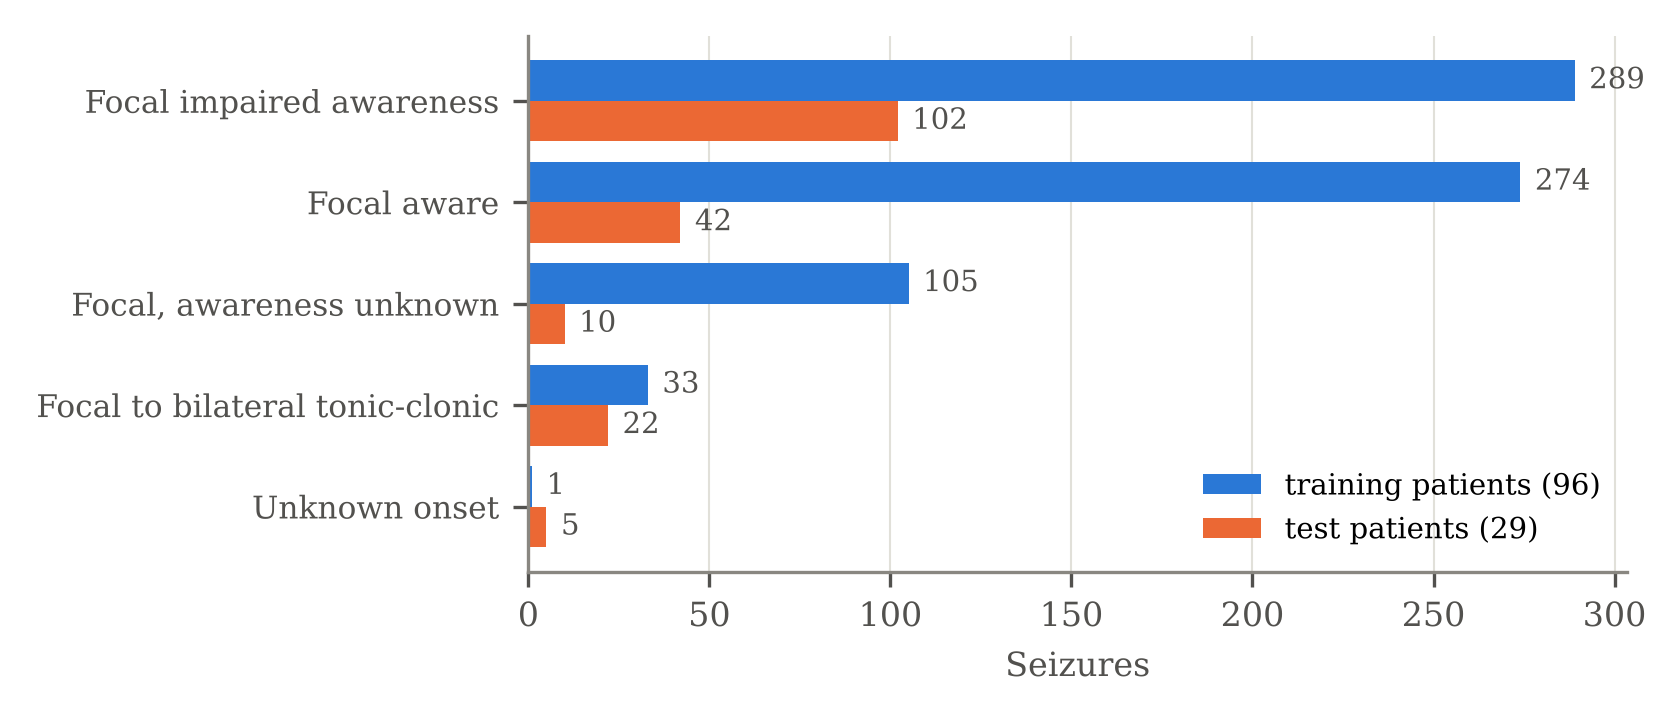
\includegraphics[width=0.78\textwidth]{figures/seizure_classes.png}
\caption{Seizure classes in the training and test patients: 822 of 883 seizures are focal seizures that do not become
tonic-clonic.}\label{fig:classes}
\end{figure}

\begin{figure}[H]
\centering
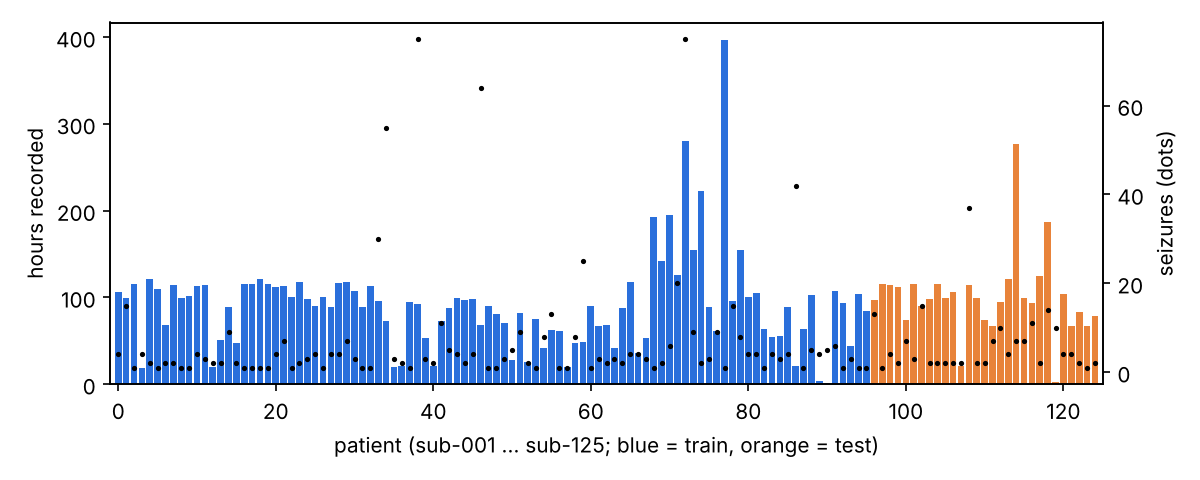
\includegraphics[width=0.9\textwidth]{figures/hours_and_seizures_per_patient.png}
\caption{Hours recorded (bars; blue: training, orange: test) and seizures per patient (dots).}\label{fig:hours}
\end{figure}

\section{Audit Findings}

\begin{table}[H]
\centering\small
\caption{Where the released files differ from the documentation, and what we did.}\label{tab:docdiff}
\begin{tabularx}{\textwidth}{@{}P{38mm}P{26mm}P{30mm}L@{}}
\toprule
\textbf{Item} & \textbf{Documentation} & \textbf{Files} & \textbf{Action}\\
\midrule
Sampling rate & 250 Hz & 256 Hz & Filters designed for 256 Hz\\
Seizures & 886 & 883 & Report our count\\
Centre and age labels & used for splits & not released & Folds by seizure count\\
Official artefact rule & 13--150\,\textmu V & flags 69\,\% of normal windows & Flags used as input bits\\
Downloads & -- & 9 files cut short & Size checks; re-extracted\\
Evaluation code & -- & two defects & Corrected values reported alongside\\
\bottomrule
\end{tabularx}
\end{table}

\section{System Architecture}

\begin{figure}[H]
\centering
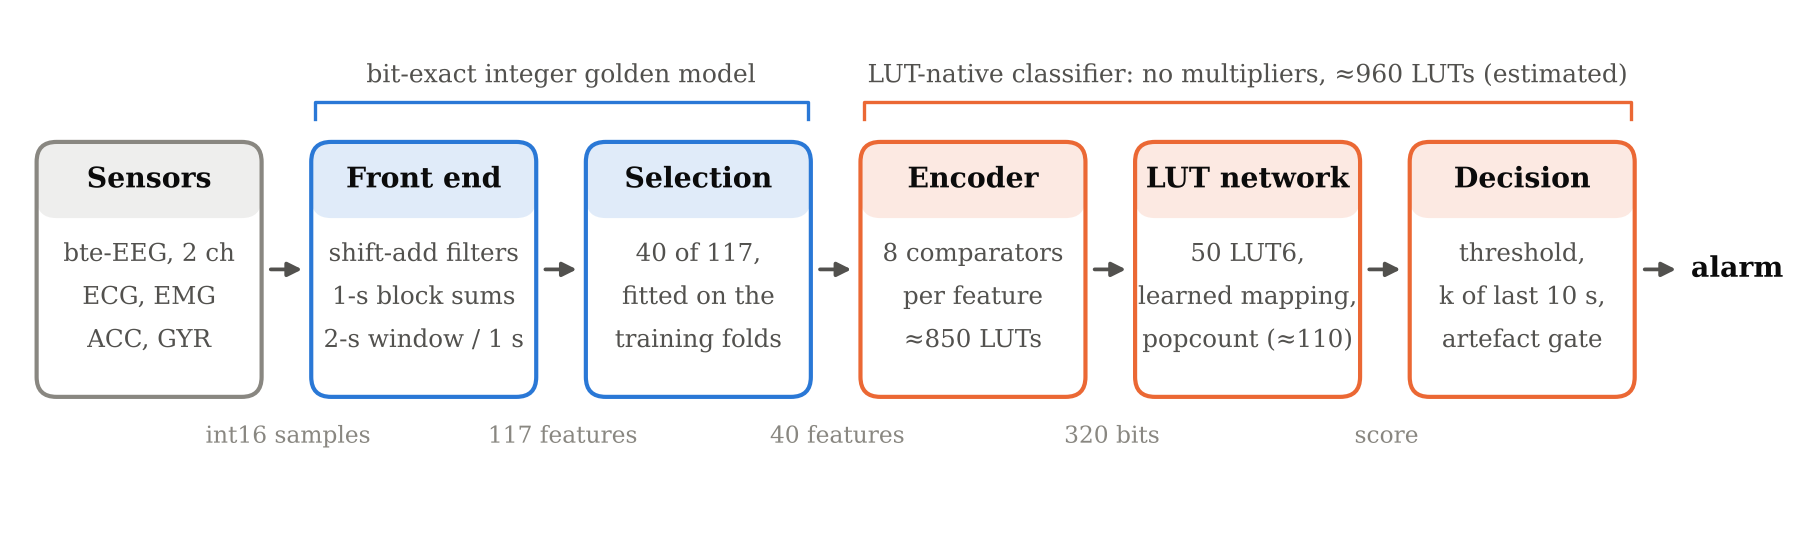
\includegraphics[width=\textwidth]{figures/system_overview.png}
\caption{The proposed detector. Blue: bit-exact integer front end; orange: LUT-native classifier.}\label{fig:system}
\end{figure}

\begin{itemize}
\item Every second, the last 2 s of all signals become \textbf{117 integer features} (Table~\ref{tab:features}).
\item The 40 most useful features are thermometer-encoded and classified by a \textbf{50-neuron LUT network}.
\item An alarm is raised when at least $k$ of the last 10 seconds are positive.
\end{itemize}

\begin{table}[H]
\centering\small
\caption{The 117 integer features (per 2-s window; many also as change from a 64-s moving average).}\label{tab:features}
\begin{tabularx}{\textwidth}{@{}lcL@{}}
\toprule
\textbf{Group} & \textbf{Count} & \textbf{Features}\\
\midrule
EEG & 84 & amplitude, line length, mobility, zero crossings, extrema, 5 band amplitudes; artefact flags\\
ECG & 5 & log heart period, log RR variability, quality flag\\
EMG & 8 & amplitude, line length, zero crossings, high/low band ratio\\
Motion & 16 & accelerometer and gyroscope magnitude, jerk, activity, band amplitude\\
Presence & 4 & one bit per sensor (ECG, EMG, accelerometer, gyroscope)\\
\bottomrule
\end{tabularx}
\end{table}

\paragraph{Integer arithmetic.} Filters use coefficients that are sums of powers of two (shifts and adds only), with
error feedback; heart rate uses $\log_2(\mathrm{RR})$, so there is no division. A floating-point twin measures the cost
of the integer arithmetic (Section~\ref{sec:intfloat}).

\section{The LUT-Native Classifier (DWN)}

A Differentiable Weightless Neural Network \cite{bacellar2024dwn} has no weights: each neuron is a 6-input truth table,
exactly one FPGA LUT.
\begin{equation}
  b_{f,i} = [\,x_f > t_{f,i}\,],\quad i = 1,\dots,8 \qquad\qquad s = \sum_{j \in S} y_j - \sum_{j \in B} y_j
\end{equation}
Each feature becomes 8 thermometer bits (one comparator each); each neuron reads 6 learned bits and outputs one stored
bit $y_j$; the score $s$ is the popcount of the seizure group $S$ minus that of the background group $B$.
Figure~\ref{fig:cost} shows the hardware cost of the final network.

\begin{figure}[H]
\centering
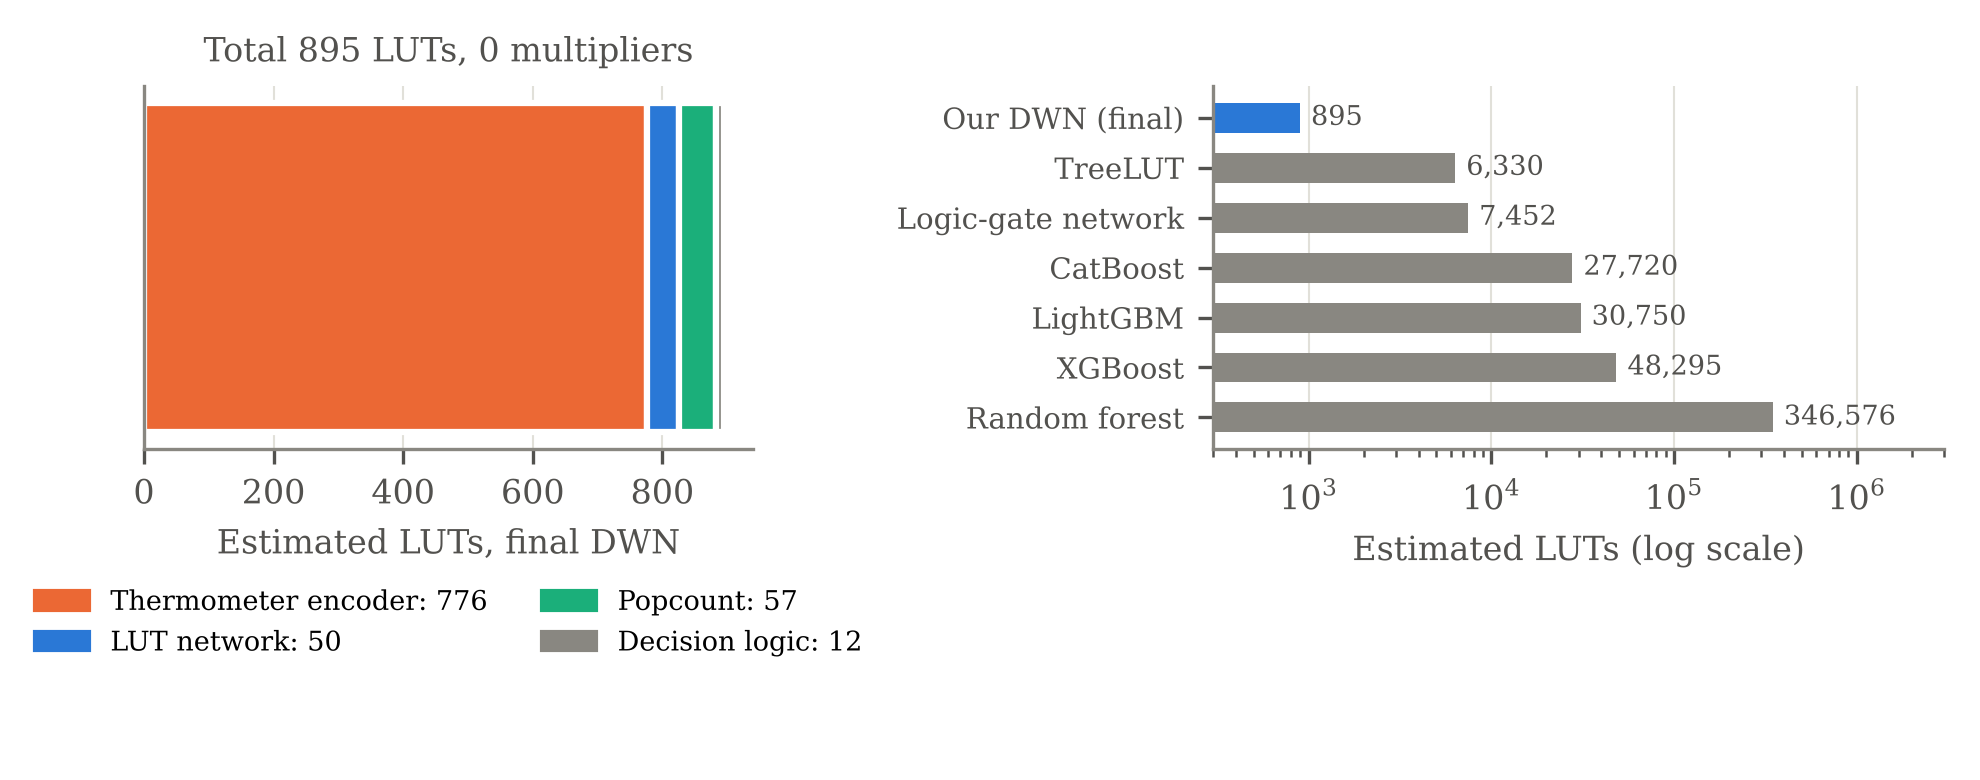
\includegraphics[width=\textwidth]{figures/cost.png}
\caption{Estimated hardware cost. Left: the final DWN by block (the encoder dominates). Right: total LUTs of each model,
log scale.}\label{fig:cost}
\end{figure}

\section{Models and Extensions}

\begin{table}[H]
\centering\small
\caption{Models compared on the same features, splits and metrics.}\label{tab:models}
\begin{tabularx}{\textwidth}{@{}P{36mm}L@{}}
\toprule
\textbf{Group} & \textbf{Models}\\
\midrule
Published baselines & ChronoNet \cite{roy2019chrononet} (CNN + GRU on raw EEG); SVM \cite{vandecasteele2020bte}\\
Software references & logistic regression, random forest, XGBoost, LightGBM, CatBoost\\
Hardware-oriented & INT8 MLP (multipliers), TreeLUT \cite{khataei2025treelut}, logic-gate network \cite{petersen2022dlgn}, DWN \cite{bacellar2024dwn}\\
\bottomrule
\end{tabularx}
\end{table}

\begin{table}[H]
\centering\small
\caption{Extensions of the DWN tested in this project (adopted only if significantly better).}\label{tab:extensions}
\begin{tabularx}{\textwidth}{@{}cL@{}}
\toprule
\textbf{ID} & \textbf{Idea}\\
\midrule
N1 & Memory across seconds: 16 state bits fed back; stacked past windows\\
N2 & Encoder design: uniform, Gaussian and learned thresholds\\
N3 & Label-free per-patient threshold adaptation\\
N4 & Distillation from LightGBM; teacher-guided hard negatives\\
N5 & Focal, noise-robust (GCE, SCE) and multiple-instance losses; onset weighting\\
N6 & Modality dropout, gated fusion, late fusion\\
N7 & Interpretability: which inputs the LUTs read during alarms\\
N8 & Post-ictal verification: a second LUT network confirms each alarm (secondary analysis)\\
\bottomrule
\end{tabularx}
\end{table}

\section{Evaluation Protocol}\label{sec:eval}

\begin{itemize}
\item \textbf{Patient-wise 5-fold cross-validation} on the 96 training patients for every design choice.
\item \textbf{Sealed test set}: the 29 test patients scored once, after the freeze, with 5 seeds; every access logged.
\item \textbf{SzCORE event scoring} \cite{dan2024szcore} (30\,s before, 60\,s after, 90\,s merge), per patient:
\end{itemize}
\begin{equation}
  \mathrm{Sens} = \frac{TP}{TP + FN},\qquad \mathrm{Prec} = \frac{TP}{TP + FP},\qquad
  F_1 = \frac{2\,\mathrm{Sens}\cdot\mathrm{Prec}}{\mathrm{Sens} + \mathrm{Prec}},\qquad \text{false alarms per 24 h}
\end{equation}
\begin{itemize}
\item \textbf{Operating points} (threshold, $k$, artefact gate) chosen on the training folds: best event-F1, and highest
  sensitivity with at most one false alarm per hour.
\item \textbf{Statistics}: paired Wilcoxon test per patient; an extension is adopted only if $p < 0.05$ in its favour.
\item \textbf{Paper metrics} (the base paper's own code) are reported for the comparison with the base paper.
\item \textbf{Compute}: a 4-core CPU server and a laptop RTX 3060 GPU.
\end{itemize}

\chapter{Experimental Results and Comparisons}\label{ch:results}

Sections~\ref{sec:res-chrononet}--\ref{sec:res-types}: development on the 96 training patients
(patient-wise cross-validation). Sections~\ref{sec:res-test}--\ref{sec:res-hw}: the single evaluation on the 29
held-out test patients, after the design was frozen.

\section{Reproduction of the Published Baseline}\label{sec:res-chrononet}

\begin{figure}[H]
\centering
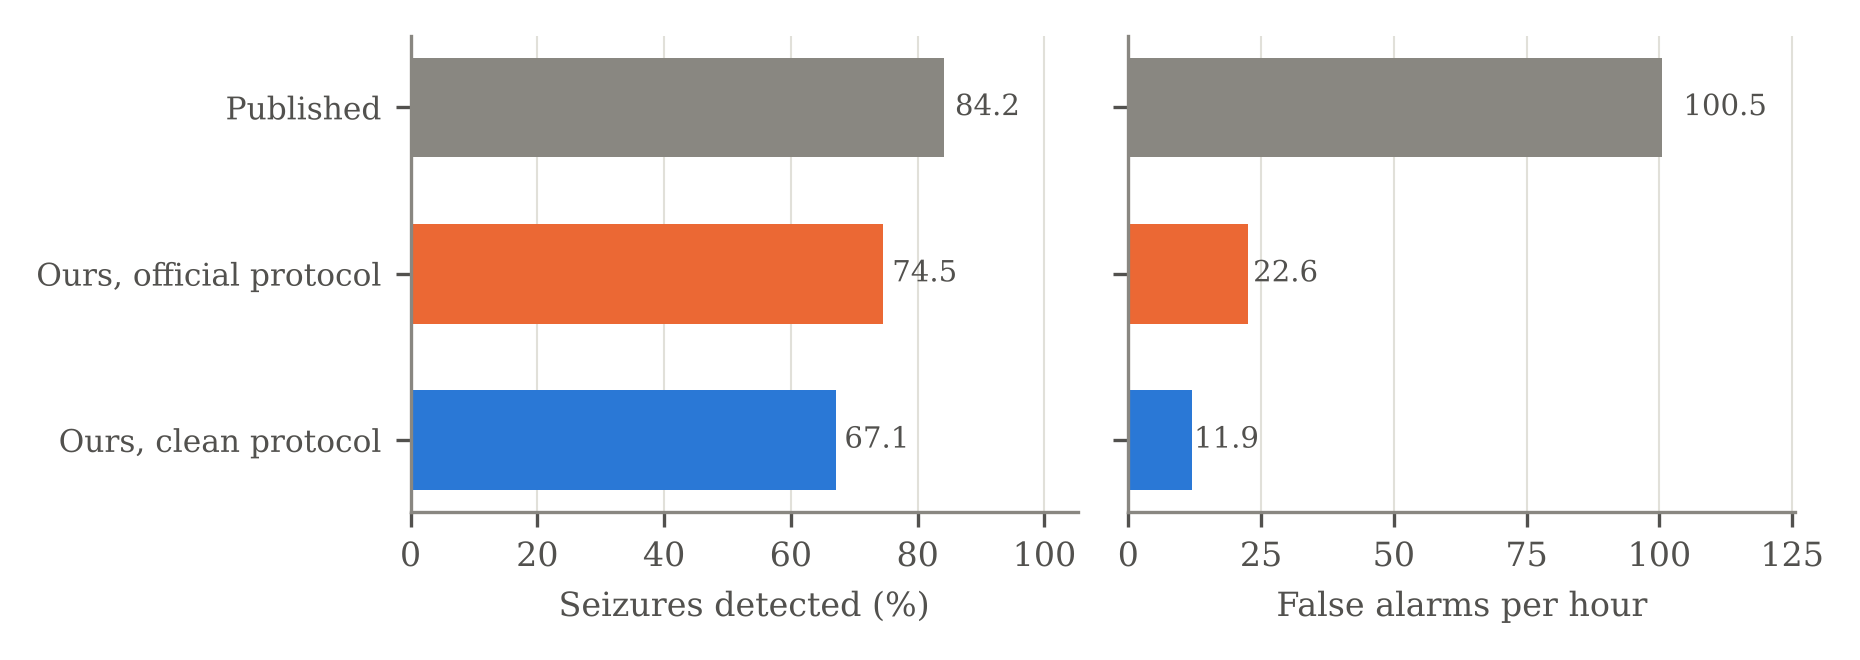
\includegraphics[width=0.9\textwidth]{figures/chrononet_repro.png}
\caption{ChronoNet on the 29 test patients: published and reproduced (the paper's metrics).}\label{fig:chrononet}
\end{figure}

\begin{itemize}
\item \textbf{Partly reproduced}: 74.5\,\% of seizures detected against 84.2\,\% published, with 22.6 instead of 100.5
  false alarms per hour (Figure~\ref{fig:chrononet}); the per-recording AUPR matches (0.109 vs 0.104).
\item \textbf{Test-set leak}: the released code picks its training epoch on the test patients. Our \textbf{clean} run
  (last epoch, no test information: 67.1\,\%, 11.9 false alarms/h) is the reference for the final comparison.
\end{itemize}

\section{Integer Versus Floating-Point Features}\label{sec:intfloat}

\begin{table}[H]
\centering\small
\caption{The integer front end against its floating-point twin (10 training patients).}\label{tab:intfloat}
\begin{tabular}{@{}lc@{}}
\toprule
\textbf{Check} & \textbf{Result}\\
\midrule
Median feature correlation, integer vs float & 0.9965\\
Artefact flags agreeing & 99.7\,\%\\
LightGBM AUROC, integer vs float features & 0.736 vs 0.735\\
\bottomrule
\end{tabular}
\end{table}

\section{Comparison of Model Families}\label{sec:res-families}

\begin{table}[H]
\centering\small
\caption{Five-fold cross-validation on the 96 training patients (best-F1 operating point).}\label{tab:families}
\begin{tabularx}{\textwidth}{@{}P{38mm}ccccL@{}}
\toprule
\textbf{Model} & \textbf{AUROC} & \textbf{Event-F1} & \textbf{FA / 24 h} & \textbf{Sens.\ at $\le$1 FA/h} & \textbf{Estimated cost}\\
\midrule
LightGBM & 0.870 & 0.292 & 3.6 & 0.594 & $\approx$30.6k LUTs\\
CatBoost & 0.863 & 0.286 & 3.0 & 0.618 & $\approx$27.7k LUTs\\
XGBoost & 0.867 & 0.277 & 3.4 & 0.603 & $\approx$47.9k LUTs\\
TreeLUT & 0.857 & 0.266 & 4.2 & 0.619 & $\approx$6.4k LUTs\\
\textbf{DWN + distillation (final)} & 0.851 & \textbf{0.229} & \textbf{0.9} & 0.597 & \textbf{$\approx$870 LUTs}\\
DWN base & 0.840 & 0.211 & 2.4 & 0.581 & $\approx$960 LUTs\\
Random forest & 0.852 & 0.198 & 0.5 & 0.536 & $\approx$323k LUTs\\
Logic-gate network & 0.843 & 0.171 & 4.9 & 0.540 & $\approx$7.5k LUTs\\
INT8 MLP & 0.830 & 0.147 & 7.8 & 0.520 & 9,600 multiplications\\
Logistic regression & 0.806 & 0.105 & 8.8 & 0.409 & 117 multiplications\\
\bottomrule
\end{tabularx}
\end{table}

\begin{figure}[H]
\centering
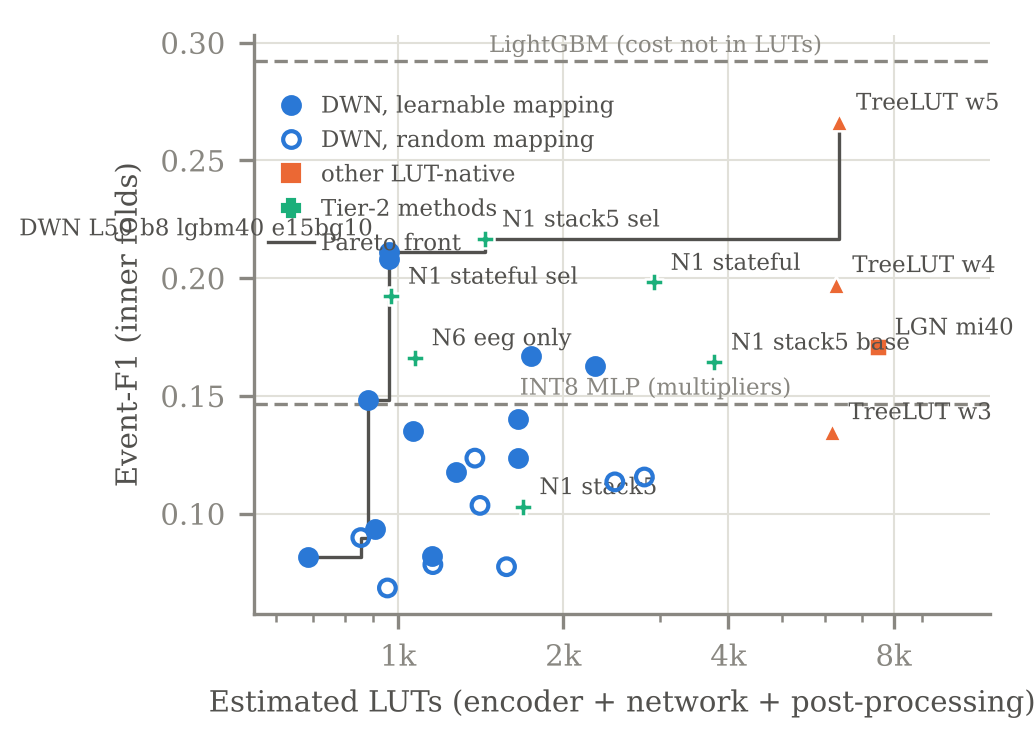
\includegraphics[width=0.68\textwidth]{figures/pareto_inner_cv.png}
\caption{Event-F1 against estimated LUTs for every LUT-native run (training folds), with the Pareto front.}\label{fig:pareto}
\end{figure}

\paragraph{Findings.} The DWN is 7--8$\times$ smaller than the other LUT models and beats the INT8 MLP on every metric
(Table~\ref{tab:families}). Larger networks (up to 2,000 LUTs), 16 thresholds, two layers and other temperatures gave no
significant gain (Figure~\ref{fig:pareto}); 4-input LUTs and 4 thresholds were clearly worse.

\section{What Improved the Network}\label{sec:res-ext}

\begin{figure}[H]
\centering
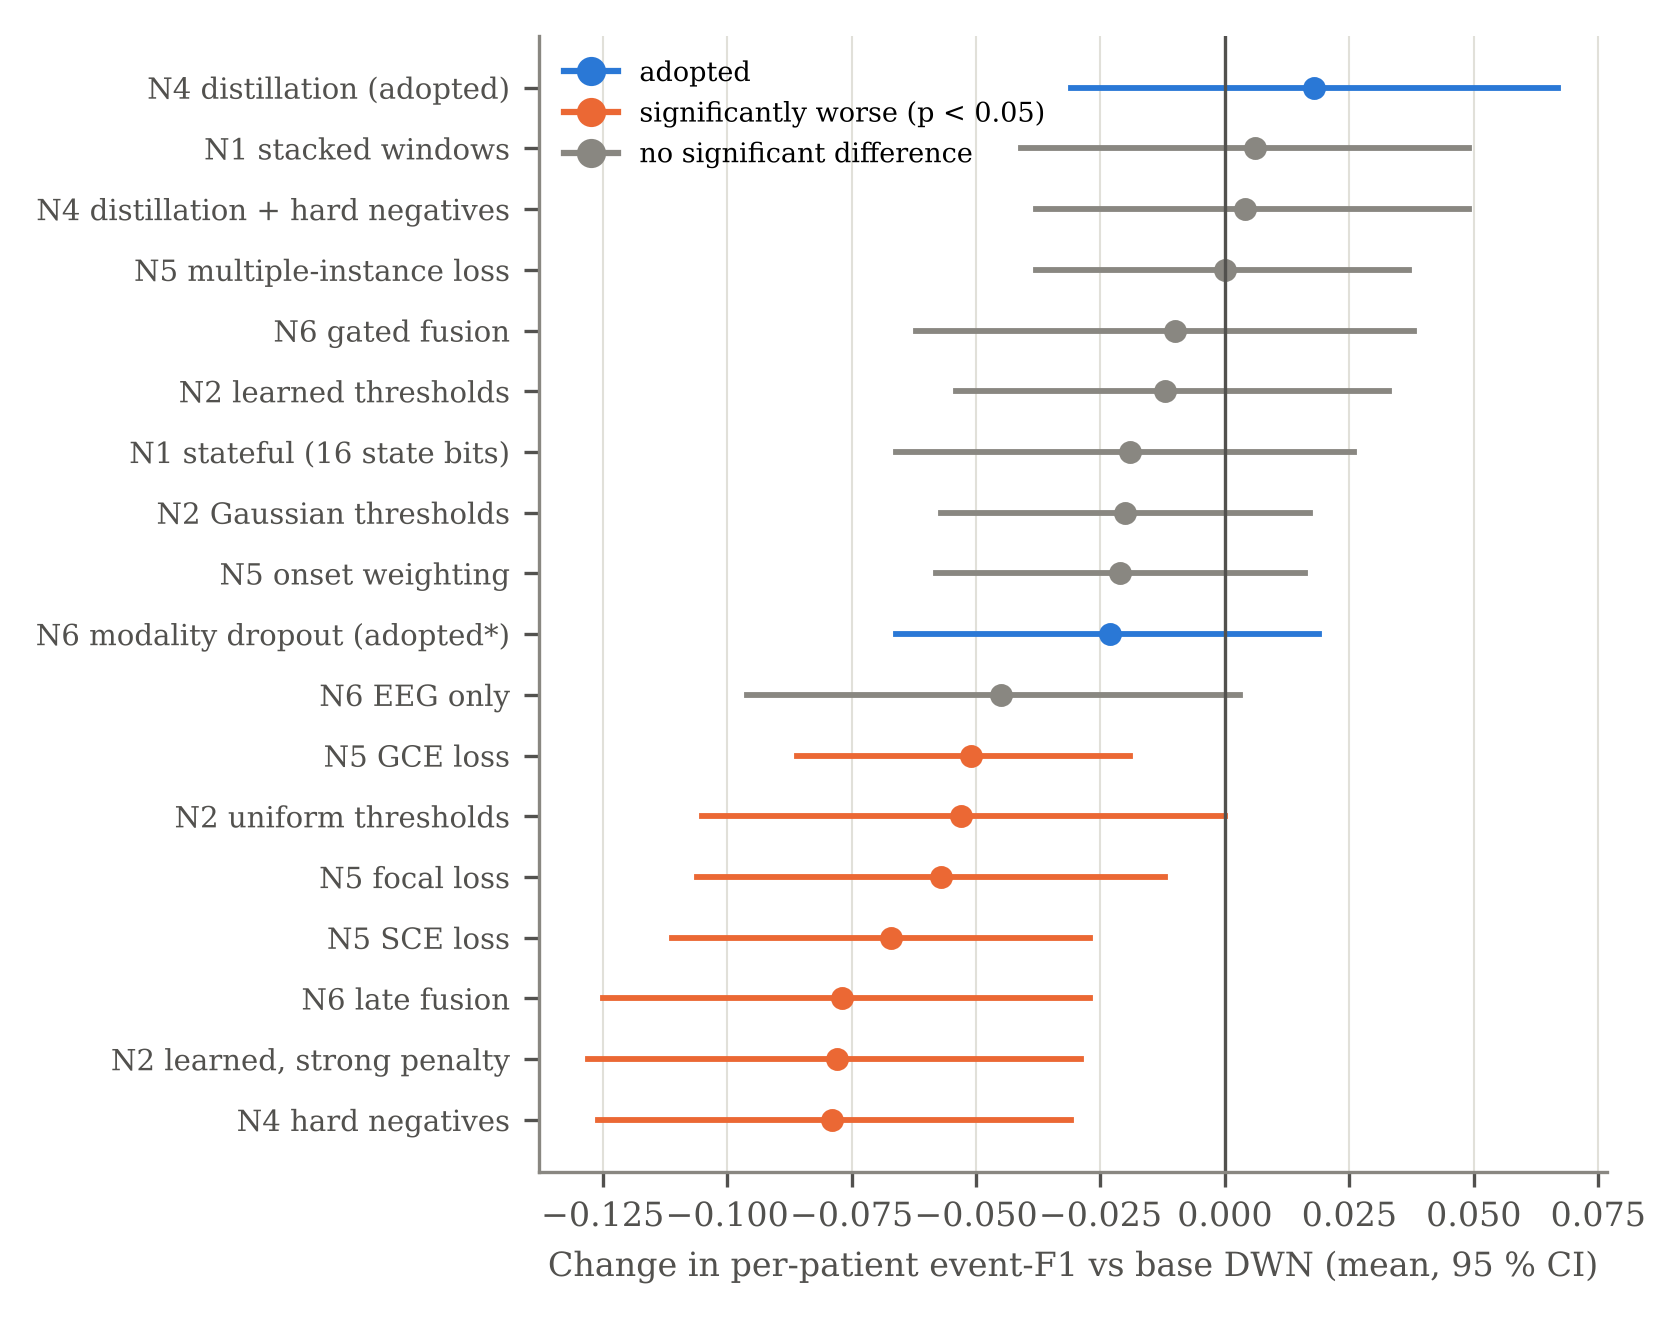
\includegraphics[width=0.85\textwidth]{figures/ablation.png}
\caption{Every extension against the base DWN: mean change in per-patient event-F1 with 95\,\% interval. *Modality
dropout was adopted for its robustness to missing sensors (Section~\ref{sec:res-missing}).}\label{fig:ablation}
\end{figure}

\begin{table}[H]
\centering\small
\caption{The changes that passed the significance test.}\label{tab:adopted}
\begin{tabularx}{\textwidth}{@{}P{42mm}LP{38mm}@{}}
\toprule
\textbf{Change} & \textbf{Evidence (training patients)} & \textbf{How it was found}\\
\midrule
Feature selection by LightGBM importance & event-F1 0.148 $\to$ 0.208 ($p = 0.047$); false alarms 7.0 $\to$ 2.3/day & N7 showed the network ignored heart rate\\
Distillation from LightGBM (\textbf{final}) & false alarms 2.4 $\to$ 0.9/day ($p = 3\times10^{-7}$); event-F1 0.229 vs 0.211 & N4\\
Modality dropout (variant) & without ECG: event-F1 0.092 $\to$ 0.172 ($p = 0.005$) & N6\\
\bottomrule
\end{tabularx}
\end{table}

\begin{figure}[H]
\centering
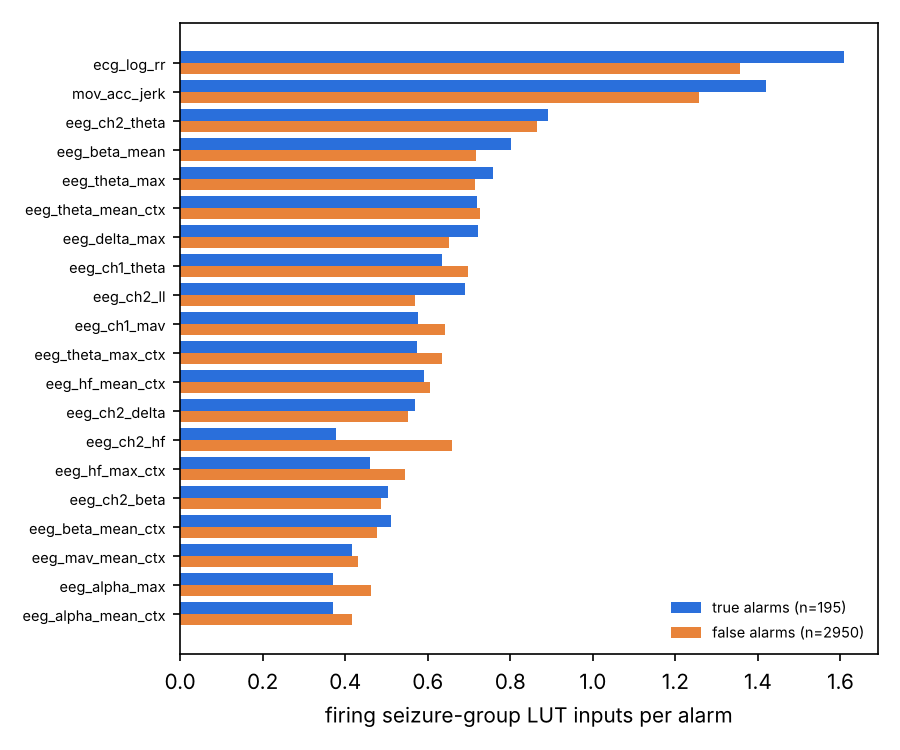
\includegraphics[width=0.55\textwidth]{figures/n7_feature_usage.png}
\caption{N7: inputs read by the firing seizure LUTs during true and false alarms (first, mutual-information network):
false alarms look like seizures to it.}\label{fig:n7}
\end{figure}

\section{Missing Sensors}\label{sec:res-missing}

\begin{figure}[H]
\centering
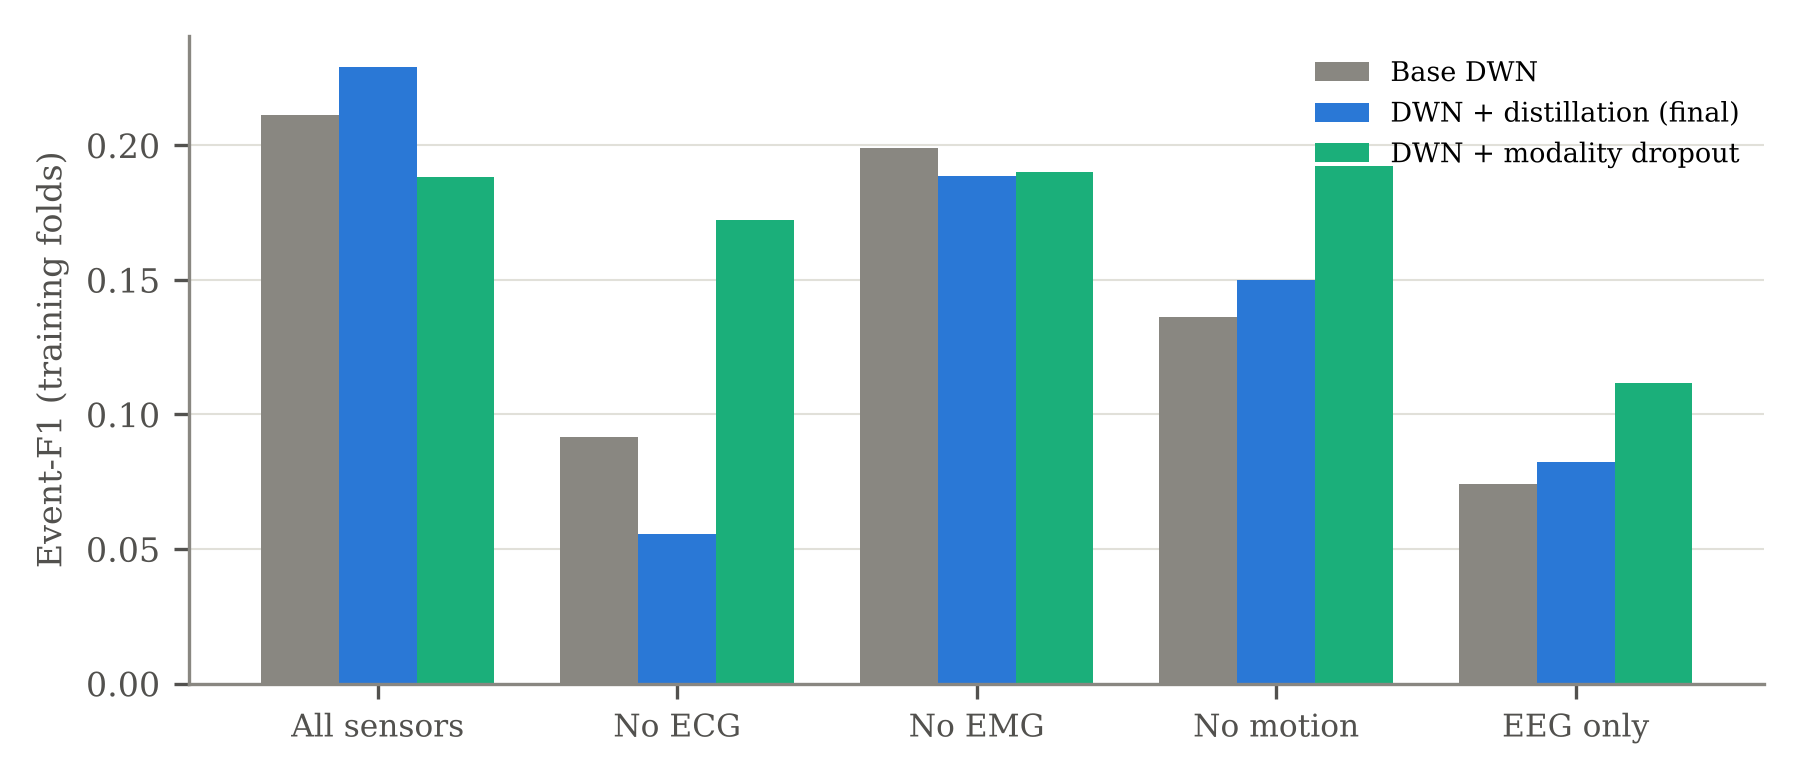
\includegraphics[width=0.85\textwidth]{figures/missing_sensors.png}
\caption{Event-F1 with sensors removed at test time (training folds). Distillation is the most accurate with all
sensors; modality dropout keeps working without ECG or motion.}\label{fig:missing}
\end{figure}

\section{Seizure Types}\label{sec:res-types}

\begin{figure}[H]
\centering
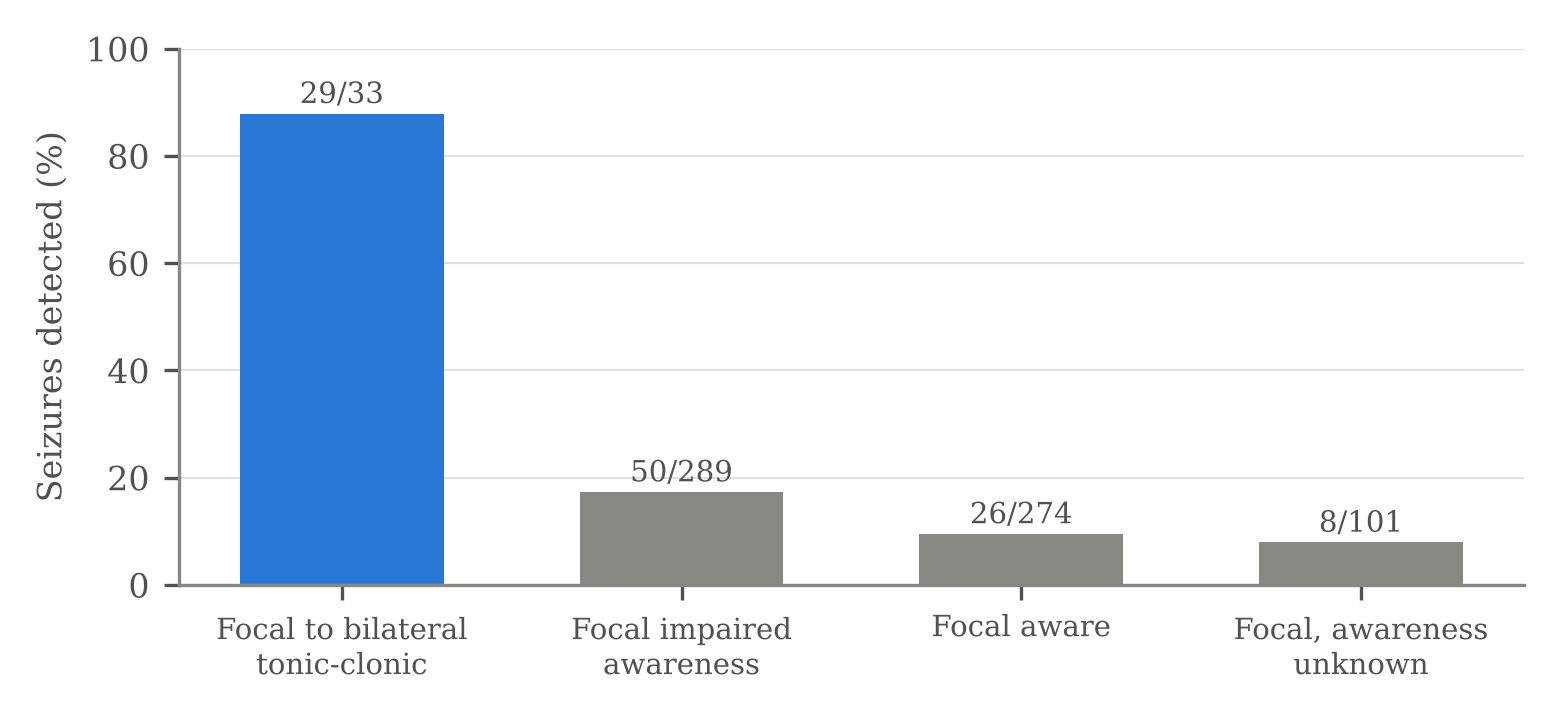
\includegraphics[width=0.65\textwidth]{figures/seizure_types.png}
\caption{Seizures detected by type (base DWN, training folds): tonic-clonic seizures are caught, focal seizures rarely.}\label{fig:types}
\end{figure}

\section{Final Evaluation on the Held-Out Test Patients}\label{sec:res-test}

\begin{figure}[H]
\centering
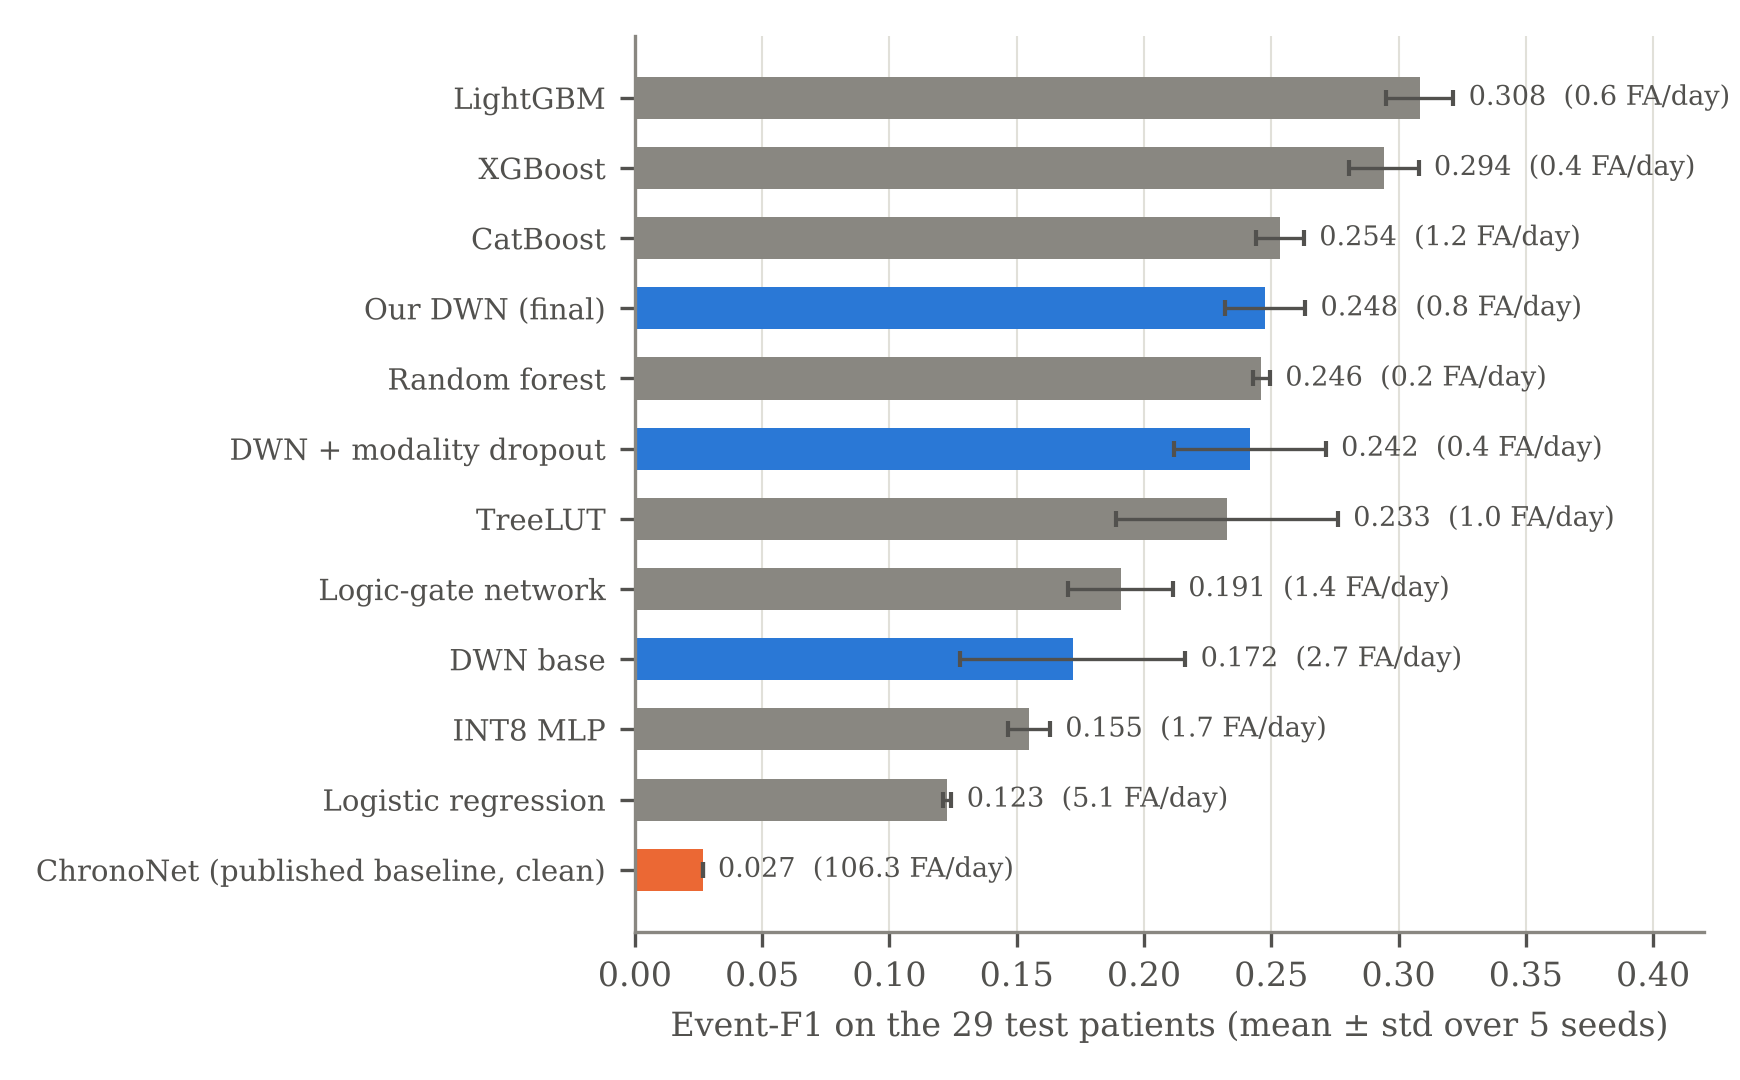
\includegraphics[width=0.85\textwidth]{figures/test_f1.png}
\caption{Event-F1 on the 29 test patients (mean $\pm$ std over 5 seeds) and false alarms per day.}\label{fig:testf1}
\end{figure}

\begin{figure}[H]
\centering
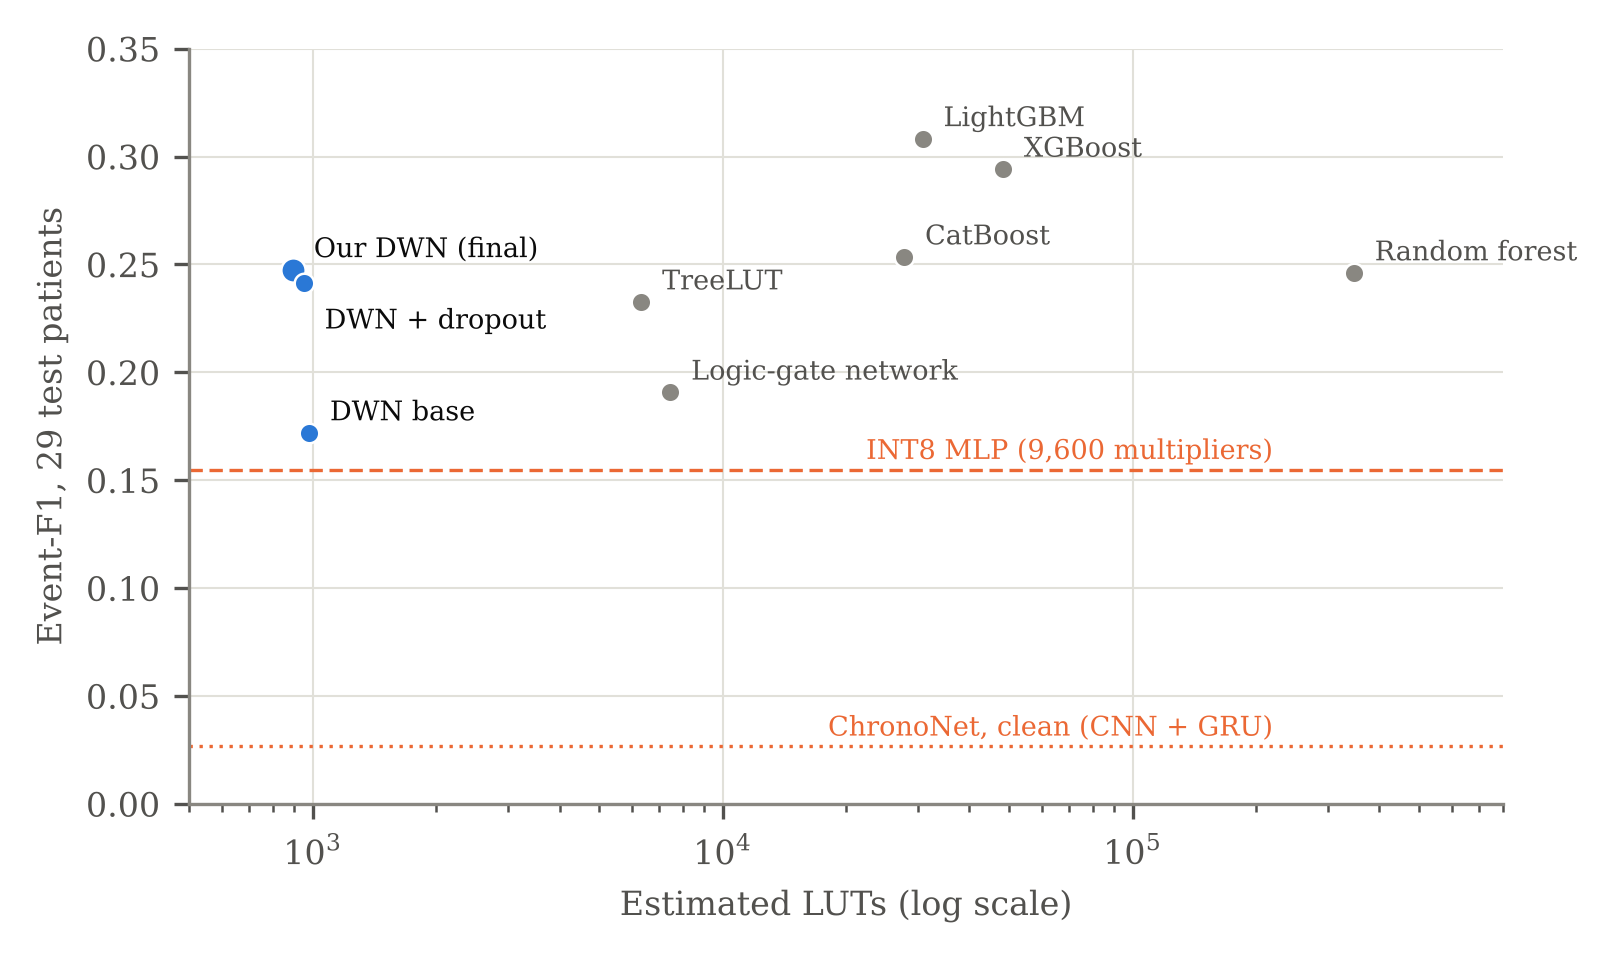
\includegraphics[width=0.8\textwidth]{figures/test_f1_vs_luts.png}
\caption{Accuracy against hardware cost on the test patients: the LUT networks reach tree-ensemble accuracy at a
fraction of the LUTs.}\label{fig:testluts}
\end{figure}

\begin{table}[H]
\centering\small
\caption[Final DWN against the main references on the 29 test patients.]{Final DWN against the main references on the 29 test patients ($p$: paired Wilcoxon on per-patient event-F1).}\label{tab:test}
\begin{tabularx}{\textwidth}{@{}P{40mm}cccL@{}}
\toprule
\textbf{Model} & \textbf{Event-F1} & \textbf{FA / 24 h} & \textbf{$p$ vs ChronoNet} & \textbf{Estimated cost}\\
\midrule
\textbf{DWN + distillation (final)} & \textbf{0.248 $\pm$ 0.016} & \textbf{0.8} & 0.027 & \textbf{$\approx$900 LUTs}\\
LightGBM & 0.308 $\pm$ 0.013 & 0.6 & 0.027 & $\approx$30.8k LUTs\\
CatBoost & 0.254 $\pm$ 0.009 & 1.2 & 0.031 & $\approx$27.7k LUTs\\
Random forest & 0.246 $\pm$ 0.003 & 0.2 & 0.27 & $\approx$347k LUTs\\
TreeLUT & 0.233 $\pm$ 0.044 & 1.0 & 0.016 & $\approx$6.3k LUTs\\
Logic-gate network & 0.191 $\pm$ 0.021 & 1.4 & 0.034 & $\approx$7.5k LUTs\\
INT8 MLP & 0.155 $\pm$ 0.008 & 1.7 & 0.017 & 9,600 multiplications\\
ChronoNet (clean) & 0.027 & 106 & -- & CNN + GRU\\
\bottomrule
\end{tabularx}
\end{table}

\paragraph{Findings.} The result held on unseen patients (0.248, above the cross-validation 0.229). The final DWN scores
above TreeLUT, the logic-gate network and the INT8 MLP, is level with random forest and CatBoost at 30--390$\times$ fewer
LUTs, and is significantly better than ChronoNet; LightGBM remains ahead ($p = 0.039$). All 11 models are in
Table~\ref{tab:test-full} (Appendix~\ref{app:sources}).

\section{Comparison with the Base Paper}\label{sec:res-published}

\begin{figure}[H]
\centering
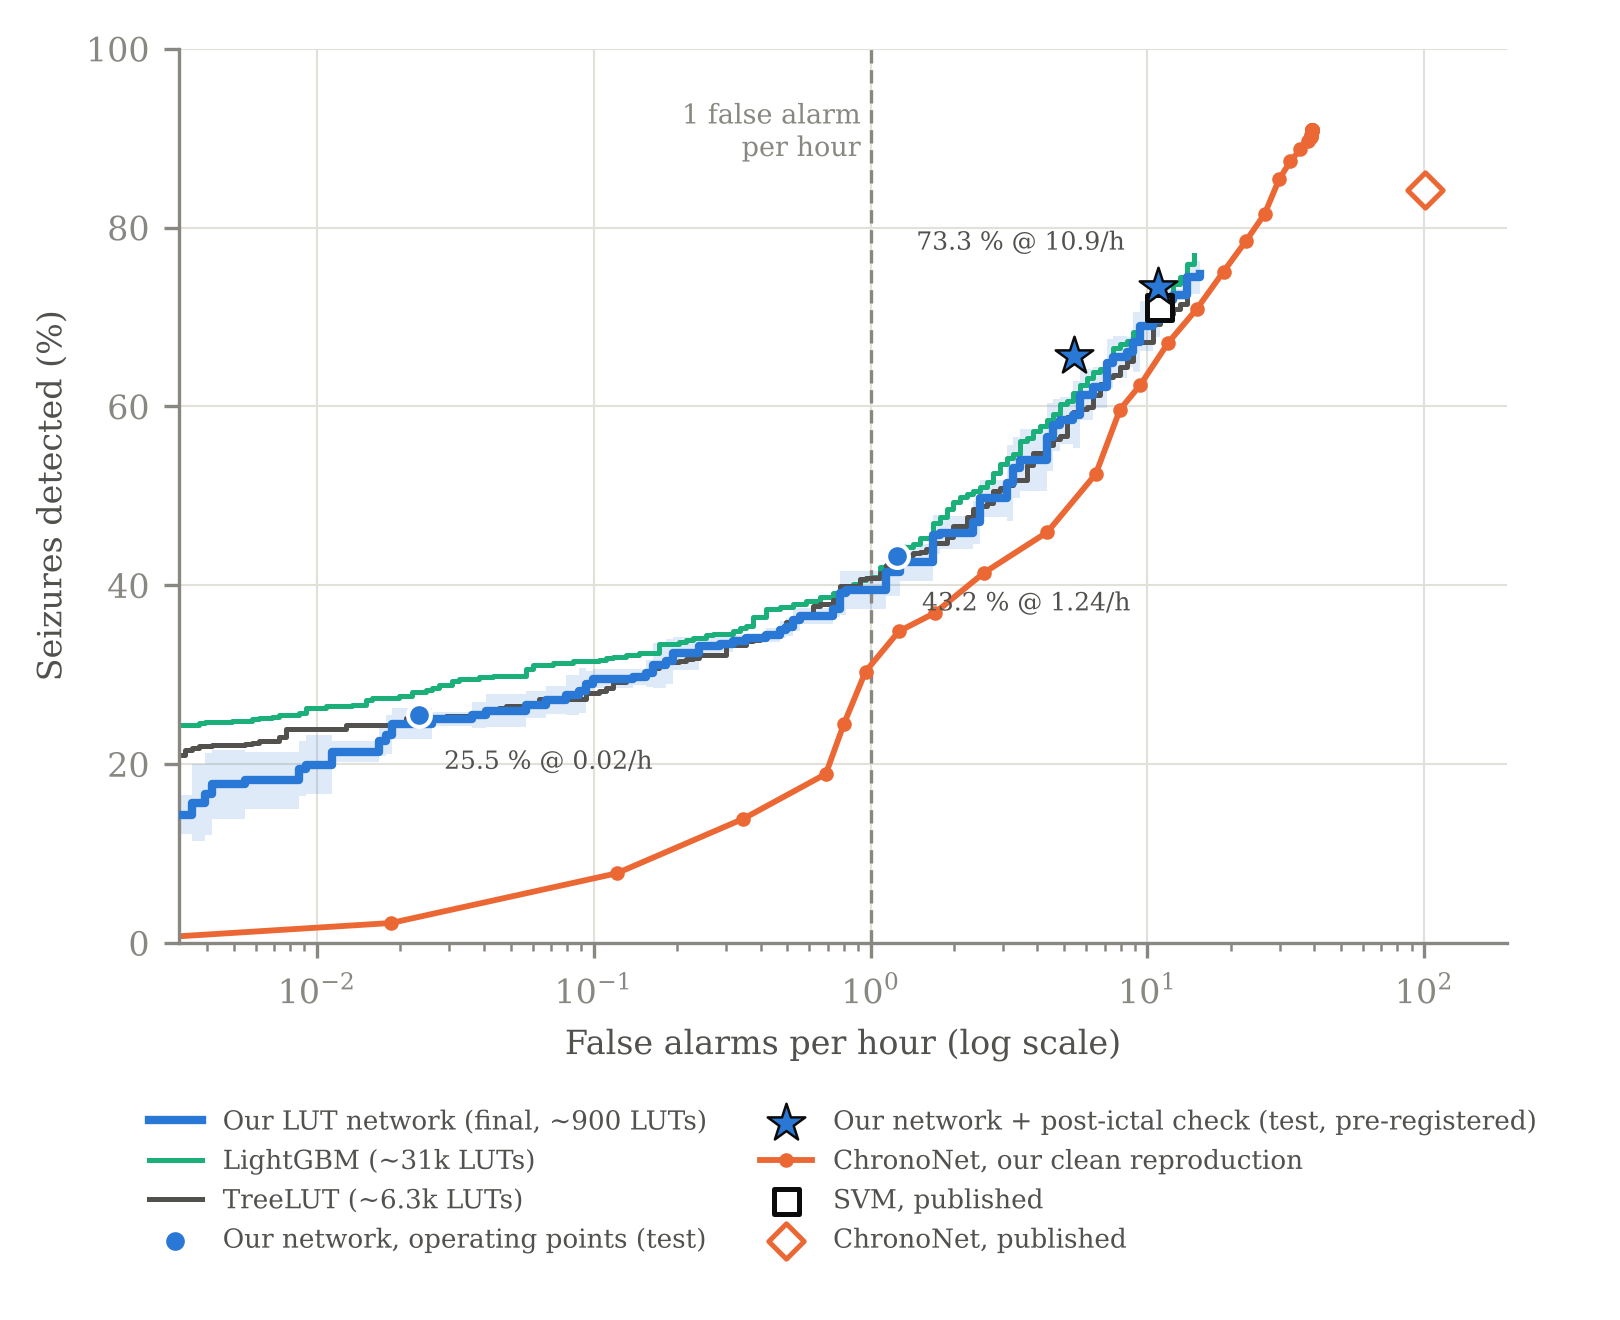
\includegraphics[width=0.85\textwidth]{figures/sens_fa_test.png}
\caption{Seizures detected against false alarms per hour on the 29 test patients (the base paper's metrics). Curves:
threshold sweeps of the frozen models (mean of 5 seeds; band: std of our network), drawn as far as every seed's sweep
reaches; dots: our two operating points, chosen on the training folds; stars: the two-stage detector
(Section~\ref{sec:res-n8}); open markers: published values.}\label{fig:sensfa}
\end{figure}

\begin{table}[H]
\centering\small
\caption{The base paper's baselines and our network on the same 29 test patients (the paper's metrics).}\label{tab:published}
\begin{tabularx}{\textwidth}{@{}P{70mm}ccL@{}}
\toprule
\textbf{Model} & \textbf{Detected} & \textbf{FA / h} & \textbf{AUROC}\\
\midrule
SVM, published \cite{bhagubai2025seizeit2} & 71.1\,\% & 11.0 & 0.700\\
ChronoNet, published \cite{bhagubai2025seizeit2} & 84.2\,\% & 100.5 & 0.792\\
ChronoNet, our clean reproduction & 67.1\,\% & 11.9 & 0.746\\
ChronoNet at $\approx$1.3 FA/h$^{*}$ & 34.8\,\% & 1.26 & --\\
\textbf{Our DWN, $\le$1 FA/h operating point} & \textbf{43.2\,\%} & \textbf{1.24} & \textbf{0.883}\\
\textbf{Our DWN, best-F1 operating point} & \textbf{25.5\,\%} & \textbf{0.02} & \\
\textbf{Our DWN + post-ictal check (pre-registered)$^{\dagger}$} & \textbf{73.3\,\%} & \textbf{10.9} & \\
\textbf{Same, stricter verification$^{\dagger}$} & \textbf{65.6\,\%} & \textbf{5.4} & \\
\bottomrule
\multicolumn{4}{@{}p{\textwidth}@{}}{\footnotesize $^{*}$ threshold read from ChronoNet's own test curve (favours it); at
0.02 FA/h ChronoNet detects 2.2\,\%. AUROC pooled over test windows; the published 0.792 uses an unreproduced definition.
$^{\dagger}$ Secondary analysis after the final test (Section~\ref{sec:res-n8}); 96\,s decision delay.}
\end{tabularx}
\end{table}

\paragraph{Findings.} The paper's baselines run at 11--100 false alarms per hour. At the same false-alarm rate our
network detects more seizures than ChronoNet (43.2\,\% vs 34.8\,\% at $\approx$1.25/h; 25.5\,\% vs 2.2\,\% at
$\approx$0.02/h), ranks windows better (AUROC 0.883 vs 0.746), and needs no multipliers. At the SVM's rate of 11 false
alarms per hour its curve reaches 69.7\,\% (SVM, published: 71.1\,\%), level with LightGBM (70.5\,\%) at 3\,\% of its
LUTs; this value is read from the test curve itself and is therefore optimistic.

\section{Post-Ictal Verification (Secondary Analysis)}\label{sec:res-n8}

Requested after the final test: detect more seizures than the base paper at slightly fewer false alarms. A two-stage
detector (N8) runs the final network at a sensitive threshold and confirms each alarm 96\,s later with a second LUT
network (50 LUTs) that compares the alarm with the minutes before and after it (EEG, heart rate, EMG, motion). All
settings were chosen on the training patients and committed before one evaluation on the test patients.

\begin{table}[H]
\centering\small
\caption[Two-stage detector with post-ictal verification.]{Two-stage detector: training patients (cross-validation) and test patients (5 seeds, paper's metrics).}\label{tab:n8}
\begin{tabular}{@{}lcccc@{}}
\toprule
\textbf{Detector} & \multicolumn{2}{c}{\textbf{Training (CV)}} & \multicolumn{2}{c}{\textbf{Test}}\\
 & Detected & FA/h & Detected & FA/h\\
\midrule
Final network, lower threshold & 74.2\,\% & 8.5 & 66.4 $\pm$ 2.0\,\% & 7.6\\
\textbf{+ post-ictal check ($\le$10 FA/h)} & 81.9\,\% & 9.6 & \textbf{73.3 $\pm$ 1.4\,\%} & \textbf{10.9}\\
+ post-ictal check ($\le$5 FA/h) & 72.3\,\% & 4.8 & 65.6 $\pm$ 1.0\,\% & 5.4\\
SVM, published \cite{bhagubai2025seizeit2} & -- & -- & 71.1\,\% & 11.0\\
\bottomrule
\end{tabular}
\end{table}

\paragraph{Findings.} At the SVM's false-alarm rate (10.9 vs 11.0 per hour) the LUT-native two-stage detector detects
2.2 points more seizures (all 5 seeds above 71.1\,\%; a small margin against a single published value). Verification
adds 3.6--6.5 points over the network alone at the same false-alarm rate. Costs: a 96\,s decision delay (seizure
logging, not instant alarms) and many false alarms per day, as for the paper's baselines; the low-false-alarm result of
Section~\ref{sec:res-test} remains the primary one.

\section{Hardware Handoff Check}\label{sec:res-hw}

\begin{table}[H]
\centering\small
\caption{Verilog of the final DWN against the software on 10 test recordings.}\label{tab:verilog}
\begin{tabular}{@{}ll@{}}
\toprule
\textbf{Item} & \textbf{Result}\\
\midrule
Exported & thresholds, input mapping, 50 truth tables, popcount head\\
Test vectors & raw samples, features, bits, LUT outputs, scores, alarms\\
Windows simulated (Icarus Verilog) & 431,960\\
Mismatches & \textbf{0}\\
\bottomrule
\end{tabular}
\end{table}

\chapter{Challenges Faced and How They Were Addressed}\label{ch:challenges}

This chapter describes the main problems met in Phase I and how each was solved. Every decision is recorded with its
evidence in the project's decision log, including the ideas that did not work.


\section{Data}

\begin{xltabular}{\textwidth}{@{}P{32mm}LL@{}}
\caption{Challenges with the data.}\label{tab:ch-data}\\
\toprule
\textbf{Challenge} & \textbf{What happened} & \textbf{How we addressed it}\\
\midrule
\endfirsthead
\toprule
\textbf{Challenge} & \textbf{What happened} & \textbf{How we addressed it}\\
\midrule
\endhead
\bottomrule
\endlastfoot
\small The data did not match its documentation & \small The paper says 250 Hz and 886 seizures; the files say 256 Hz
and 883. Centre and age labels, needed for stratified splits, are not in the public release; seizure-visibility labels
are empty. & \small A full audit of all 11,009 files before any modelling. Every window and filter is defined in
seconds and designed for 256 Hz; folds are stratified by seizure count; analyses the data cannot support were dropped
and reported.\\
\small 126 GB of data on a machine without the disk or a GPU & \small The dataset could not be stored where the code
runs. & \small The audit and the feature extraction stream each file from the public S3 bucket, process it and delete
it; only the 3.5 GB of integer features are kept.\\
\small Silent download truncation & \small Comparing integer and floating-point features exposed one ECG file cut at
51,855 of 71,835 s. A new verifier then found 9 recordings silently truncated by incomplete network reads (one EEG file
had 12 of 16,363 windows). & \small Downloads are now checked against the expected size and every cached recording
against the audit durations. All 9 were re-extracted, and the 3 model runs trained on the bad cache were repeated.\\
\small A recording with an ECG lead but no detectable heartbeat & \small The feature extractor crashed on an empty list
of beats (3,250 s of data). & \small The recording is kept, its ECG features are set to 0 and a quality bit is
raised.\\
\small The official artefact rule does not suit behind-the-ear EEG & \small The 13\,\textmu V RMS floor flags 69\,\% of
ordinary windows on one channel, because behind-the-ear amplitudes are close to it. & \small For our models the
artefact flags are input bits, and whether to gate alarms on them is chosen on the training folds.\\
\end{xltabular}

\section{Reproducing the Published Baseline}

\begin{xltabular}{\textwidth}{@{}P{32mm}LL@{}}
\caption{Challenges in reproducing the published baseline.}\label{tab:ch-repro}\\
\toprule
\textbf{Challenge} & \textbf{What happened} & \textbf{How we addressed it}\\
\midrule
\endfirsthead
\toprule
\textbf{Challenge} & \textbf{What happened} & \textbf{How we addressed it}\\
\midrule
\endhead
\bottomrule
\endlastfoot
\small ChronoNet did not reproduce & \small Our run detected 74.5\,\% of seizures against 84.2\,\% published, with 22.6
instead of 100.5 false alarms per hour. & \small We ported the official code literally (identical outputs on 900 random
test cases) and then checked the metric definitions: the published AUPR matches only when averaged per recording
(0.109 against 0.104), and the published false-alarm rate matches neither definition in the code. The gap is reported
as measured.\\
\small The released code selects its model on the test patients & \small Its training loop keeps the epoch with the
best score on the same patients it is then evaluated on. & \small We reproduced it as published and also trained a
clean version (last epoch, no test information), which is the honest reference for the final comparison.\\
\small Defects in the released evaluation code & \small True positives can be counted more than once, and the artefact
gate (\texttt{a and b} on two Python lists) silently uses only one channel. & \small Reproduced as written for the
comparison with the paper; corrected numbers reported in a separate column.\\
\small The SVM baseline cannot be rebuilt yet & \small The dataset paper defers its 42 features to Vandecasteele et al.\
\cite{vandecasteele2020bte}, whose full text was not available to us. & \small Still open: we need that paper's feature
table.\\
\end{xltabular}

\section{Hardware Arithmetic}

\begin{xltabular}{\textwidth}{@{}P{32mm}LL@{}}
\caption{Challenges with the integer (hardware) arithmetic.}\label{tab:ch-hw}\\
\toprule
\textbf{Challenge} & \textbf{What happened} & \textbf{How we addressed it}\\
\midrule
\endfirsthead
\toprule
\textbf{Challenge} & \textbf{What happened} & \textbf{How we addressed it}\\
\midrule
\endhead
\bottomrule
\endlastfoot
\small Rounding noise in integer filters & \small With plain rounding, the 0.5 Hz high-pass filter had an error of 140
LSB standard deviation, larger than the signal itself (61 LSB). & \small Second-order error feedback of the discarded
bits reduced the error to 0.7 LSB.\\
\small Quantised coefficients moved the filter zeros & \small Rounding each coefficient independently moved the
low-pass zeros away from the Nyquist frequency (stop-band floor $-55$ dB). & \small Structure-preserving quantisation,
$b = b_0\,(1, \pm 2, 1)$, with coefficients as sums of powers of two.\\
\small Heart rate without a divider & \small Heart rate needs $60/\mathrm{RR}$. & \small We use
$\log_2(\mathrm{RR})$ from integer R-peak timestamps: no division and no multiplication.\\
\small Proving that the integer pipeline costs nothing & \small Hardware arithmetic could lose accuracy silently. &
\small A floating-point twin of every feature: median correlation 0.9965 and equal LightGBM AUROC (0.736 against
0.735).\\
\small TreeLUT scores were not comparable across folds & \small Each fold's integer score had its own scale, so pooled
thresholds were meaningless; 3-bit leaves could not represent the model. & \small Scores converted to a common unit;
leaf width chosen on the folds (5 bits).\\
\small Verilog disagreed with the software & \small Thresholds outside a feature's bit width (for example 79 on a 2-bit
presence feature) produced wrong comparator logic. & \small The Verilog generator now emits constant bits for such
thresholds; the simulation agrees with the software on 100\,\% of the test vectors.\\
\end{xltabular}

\section{Computing and Infrastructure}

\begin{xltabular}{\textwidth}{@{}P{32mm}LL@{}}
\caption{Challenges with computing resources.}\label{tab:ch-infra}\\
\toprule
\textbf{Challenge} & \textbf{What happened} & \textbf{How we addressed it}\\
\midrule
\endfirsthead
\toprule
\textbf{Challenge} & \textbf{What happened} & \textbf{How we addressed it}\\
\midrule
\endhead
\bottomrule
\endlastfoot
\small Limited GPU resources & \small Our GPU is a laptop RTX 3060 with 6 GB of memory and 7.4 GB of system memory,
and the reference DWN library runs only on CUDA. & \small We re-implemented the DWN in PyTorch, identical to the
library's CUDA kernel (unit-tested), so that it also runs on CPUs. CPU jobs run on a 4-core server; large networks and
raw-EEG models run on the GPU.\\
\small Long runs interrupted & \small Machine restarts stopped long runs; the logic-gate network lost 3 of its 5
folds once. & \small Every run resumes at fold and epoch level, and a queue skips finished runs; a resumed run was
checked to give identical metrics.\\
\small Out-of-memory failures & \small The stateful network's sequence sampler held 24 million windows in memory
(13.9 GB of a 15 GB machine). & \small A new sampler reads each recording once and stores bits as bytes: the same
sequences with a peak of 3.1 GB.\\
\small Two machines, one code base & \small The CPU server and the GPU laptop must not overwrite each other's work. &
\small One version-controlled code base, written run instructions for each machine, and automatic tests on every
change.\\
\end{xltabular}

\section{Machine Learning}

\begin{xltabular}{\textwidth}{@{}P{32mm}LL@{}}
\caption{Challenges in the machine-learning design.}\label{tab:ch-ml}\\
\toprule
\textbf{Challenge} & \textbf{What happened} & \textbf{How we addressed it}\\
\midrule
\endfirsthead
\toprule
\textbf{Challenge} & \textbf{What happened} & \textbf{How we addressed it}\\
\midrule
\endhead
\bottomrule
\endlastfoot
\small Seizures are 0.123\,\% of the time & \small Accuracy is meaningless, and training on all windows teaches the
model never to fire. & \small Event-based scoring (SzCORE) per patient; training on all seizure windows plus a fixed
ratio of background windows; operating points chosen for a false-alarm budget.\\
\small Results must hold on unseen patients & \small Mixing a patient's windows between training and validation
inflates results. & \small Patient-wise five-fold cross-validation; feature selection and thresholds fitted inside each
training fold only; the test patients locked behind a flag, with every access logged.\\
\small Early results were weaker than expected & \small The first LUT network, with mutual-information features,
reached an event-F1 of 0.148 with 7.0 false alarms per day; the interpretability study showed that it ignored the
heart-rate and muscle features. & \small Feature selection by LightGBM importance: event-F1 0.208 and 2.3 false alarms
per day at the same size.\\
\small A confounded comparison & \small The stateful network had received all 117 features instead of the selected 40,
so its apparent gain mixed two changes. & \small Found by checking the run's records; all models now share one training
function, and the run was repeated.\\
\small Stacking past windows picked duplicate features & \small Ranking the 585 stacked columns kept lagged copies of
only 11--13 distinct features. & \small Rank on the current window, then keep every lag of the selected features.\\
\end{xltabular}

\chapter{Discussion, Conclusions and Future Scope}\label{ch:concl}

\section{Discussion and Current Findings}

\paragraph{Accuracy per LUT.} The 50-LUT DWN gives the best accuracy per unit of hardware among the models compared:
an event-F1 of 0.211 with 2.4 false alarms per day at about 960 estimated LUTs and no multipliers, against 0.266 for
TreeLUT at about 6.4k LUTs and 0.292 for LightGBM, which is not a hardware design. The INT8 MLP, the conventional way
to put a neural network on a chip, is worse on every metric while needing 9,600 multiplications per decision. Within
the DWN family, size did not matter between 50 and 200 LUTs, while the choice of input features and the encoder
resolution did.

\paragraph{The encoder dominates the cost.} About 850 of the 960 estimated LUTs are comparators of the thermometer
encoder; the network itself is 50 LUTs. This agrees with recent measurements of DWN hardware \cite{mecik2025thermo} and
makes the encoder (extension N2) the main lever for reducing the hardware further.

\paragraph{False alarms look like seizures to the network.} The interpretability study showed that the network reads
almost the same inputs during true and false alarms. It also exposed a weakness of the first feature selection, which
ignored the heart signal; fixing it was the largest single improvement of Phase I. Inspecting the trained LUTs was
therefore more useful than tuning the network blindly.

\paragraph{Tonic-clonic against focal seizures.} The detector finds 88\,\% of tonic-clonic seizures but 8--17\,\% of
focal seizures, and loses most of its performance without ECG. This matches the literature, where wearable detection is
established only for tonic-clonic seizures \cite{beniczky2021guideline}, and it shows where the remaining work lies:
focal seizures and robustness to missing sensors.

\paragraph{Reproducibility.} The published ChronoNet baseline could only be partly reproduced, and its released code
selects the model on the test patients. Keeping our own test patients untouched until the design is frozen, and
reporting a clean version of the baseline, is therefore essential for an honest final comparison.

\section{Current Progress and Future Scope}

Table~\ref{tab:phase1-months} summarises the work carried out in the two months of Phase I, and
Table~\ref{tab:status} the status of every activity at the end of Phase I.

\begin{table}[htbp]
\centering\small
\caption{Work carried out during Phase I.}\label{tab:phase1-months}
\begin{tabularx}{\textwidth}{@{}P{30mm}L@{}}
\toprule
\textbf{Period} & \textbf{Activities}\\
\midrule
Month 1 (September 2026) & Selection of the topic and definition of the problem with the guide; literature study on
wearable seizure detection and LUT-based neural networks; study of the SeizeIT2 dataset, its baselines and its
evaluation; setting up the software tools and data access; first experiments, whose results were weaker than those
reported here.\\
Month 2 (October -- November 2026) & Complete audit of the dataset; reproduction of the ChronoNet baseline (official
and clean); integer feature pipeline and fixed-point specification; cross-validated comparison of nine model families;
design study of the DWN and the improved feature selection; first extensions (N1, N3, N7); hardware handoff tools;
this report.\\
\bottomrule
\end{tabularx}
\end{table}

\begin{xltabular}{\textwidth}{@{}P{55mm}P{26mm}L@{}}
\caption{Status of the project activities at the end of Phase I.}\label{tab:status}\\
\toprule
\textbf{Activity} & \textbf{Status} & \textbf{Remarks}\\
\midrule
\endfirsthead
\toprule
\textbf{Activity} & \textbf{Status} & \textbf{Remarks}\\
\midrule
\endhead
\bottomrule
\endlastfoot
\small Literature review & \small Completed & \small 79 references in five areas; research gaps identified\\
\small Dataset access and audit & \small Completed & \small All 11,009 files measured; differences from the
documentation recorded\\
\small Reproduction of ChronoNet & \small Completed & \small Partly reproduced; the clean run is the reference for the
final comparison\\
\small Reproduction of the SVM baseline & \small Pending & \small Needs the 42-feature definition of the original
study\\
\small Integer feature pipeline and fixed-point specification & \small Completed & \small 117 features; no measurable
accuracy loss\\
\small Comparison of model families & \small Completed for nine families & \small LogicNets-style network, GRU and
raw-EEG CNN/TCN running\\
\small DWN design study & \small Completed up to 200 LUTs & \small 500--2,000 LUTs and further ablations running on the
GPU\\
\small Extensions N1, N3, N7 & \small Completed & \small None adopted alone; N7 led to the improved feature selection\\
\small Extensions N2, N4, N5, N6 & \small In progress & \small 16 variants running; missing-sensor tests to follow\\
\small Hardware handoff tools (export, test vectors, reference Verilog) & \small Completed and tested & \small Run on
the final model in Phase II\\
\small Final evaluation on the 29 test patients & \small Planned & \small After every design choice is frozen; five
seeds per model\\
\small FPGA implementation & \small Planned & \small Synthesis, measurements and demonstration in Phase II\\
\end{xltabular}

The remaining months will concentrate on the open questions of Phase I. The extensions will be completed and the
winners combined; the large LUT networks and the raw-EEG references will close the model comparison; the design will
then be frozen and evaluated once on the 29 test patients. The final DWN will be exported as truth tables with test
vectors, implemented on a low-power FPGA and measured against the INT8 MLP and TreeLUT on the same device.
Table~\ref{tab:plan} gives the month-wise plan.

\begin{table}[htbp]
\centering\small
\caption{Month-wise plan for the remaining project period.}\label{tab:plan}
\begin{tabularx}{\textwidth}{@{}P{30mm}LP{42mm}@{}}
\toprule
\textbf{Month} & \textbf{Work} & \textbf{Expected deliverable}\\
\midrule
November -- December 2026 & Remaining extensions (N2, N4, N5, N6) and their combination; large DWNs, GRU and raw-EEG
references; design frozen & Ablation table; final DWN design\\
December 2026 & Final evaluation on the 29 test patients with five seeds; hardware handoff package & Test-set results;
handoff package with verified reference Verilog\\
January 2027 & FPGA synthesis and place-and-route; conference paper draft (EMBC 2027, full papers reportedly due 24
January 2027) & Resource and timing report; paper draft\\
February 2027 & Measured LUTs, power and latency; INT8 MLP and TreeLUT on the same device & Hardware comparison table\\
March 2027 & On-board demonstration with recordings streamed through the design; documentation & Demonstration\\
April 2027 & Final report and presentation & Final report\\
\bottomrule
\end{tabularx}
\end{table}

\section{Conclusions}

Phase I established the foundation of the project and its first results:
\begin{enumerate}
\item The SeizeIT2 dataset was audited completely; its sampling rate, seizure count and labels differ from the
  documentation, and the design follows the files.
\item The published ChronoNet baseline was reproduced only partly, and a clean version without test information was
  trained as the reference for the final comparison.
\item A bit-exact integer feature pipeline for behind-the-ear EEG, ECG, EMG and motion loses no measurable accuracy
  against floating point.
\item A 50-LUT Differentiable Weightless Neural Network reaches an event-F1 of 0.211 with 2.4 false alarms per day on
  cross-validation, at about 960 estimated LUTs and no multipliers: seven to eight times smaller than the other LUT
  models and better than an INT8 network, though still below gradient-boosted trees.
\item Interpretability of the LUT network led to the largest improvement of the phase, and the thermometer encoder was
  identified as the dominant hardware cost.
\item No LUT-native seizure detector exists in the literature, and no LUT network fuses modalities or handles missing
  sensors; the project addresses both.
\end{enumerate}
Phase II will complete the extensions, evaluate the frozen design once on the 29 held-out patients, and implement and
measure the detector on an FPGA.


% ================================================================ references and appendices
\cleardoublepage
\phantomsection
\addcontentsline{toc}{chapter}{References}
\renewcommand{\bibname}{References}
\markboth{References}{}
{\small\singlespacing
\bibliographystyle{IEEEtran}
\bibliography{refs}}

\appendix
\chapter{Sources of the Reported Numbers}\label{app:sources}

Every number in this report comes from a saved result file of the project. Table~\ref{tab:sources} lists where each
group of numbers is stored; the run folders hold the configuration, the code version, the log and the metrics of each
experiment.

\begin{xltabular}{\textwidth}{@{}P{55mm}L@{}}
\caption{Sources of the reported numbers.}\label{tab:sources}\\
\toprule
\textbf{Numbers} & \textbf{Source}\\
\midrule
\endfirsthead
\toprule
\textbf{Numbers} & \textbf{Source}\\
\midrule
\endhead
\bottomrule
\endlastfoot
\small Dataset inventory, seizure classes, differences from the documentation, signal quality (Chapter 3) &
\small \texttt{reports/data\_audit.md}, \texttt{reports/data\_audit.json}, \texttt{results/audit/}\\
\small Fixed-point specification of the features & \small \texttt{spec/fixed\_point.md}\\
\small Integer against floating-point features & \small \texttt{results/m3/int\_float\_gap.md}\\
\small ChronoNet reproduction (Table~\ref{tab:chrononet}) & \small runs \texttt{20261107-125159\_chrononet\_official\_s1}
and \texttt{20261107-204035\_chrononet\_clean\_s1}\\
\small Comparison of model families (Table~\ref{tab:families}) & \small \texttt{results/tables/inner\_cv.md} and the run
folders named there\\
\small Effect of the feature selection (Table~\ref{tab:featsel}) & \small runs \texttt{dwn\_L50\_b8\_learn} and
\texttt{dwn\_L50\_b8\_lgbm40}\\
\small Base DWN, training recipe, seizure types and missing sensors & \small run
\texttt{20261108-082813\_dwn\_L50\_b8\_lgbm40\_e15bg10\_s0} (\texttt{metrics.json}, \texttt{breakdown.md})\\
\small Extensions (Table~\ref{tab:ext-results}) & \small \texttt{results/tables/m5\_ablation.md};
\texttt{n7\_interpretability.json} and \texttt{n3\_adaptation.json} in the run folder of \texttt{dwn\_L50\_b8\_learn}\\
\small Decisions and their evidence & \small \texttt{results/decisions.md}\\
\end{xltabular}


\end{document}
